\documentclass[a4paper,12pt,oneside]{article}%FinalView
%\documentclass[draft,a4paper,12pt,oneside]{article}%draftView

\usepackage{indentfirst}

%Page Geometry
\usepackage[
	top=3cm,
	bottom=2cm,
	left=2cm,
	right=2cm,
	%bindingoffset=2cm, %Adds a Binding offset for printed documents
	marginparwidth=6cm, %Adds Overflow Width to Rigth Margin 
	marginparsep=3mm %Gap between right margin and right overflow margin
	]{geometry}
%\usepackage{showframe} % UNCOMMENT TO SHOW BORDERS REPRESENTING YOUR PAGE ARANGMENT
%\usepackage[cam,center,a3]{crop}%Extends PageView

\usepackage[T1]{fontenc}
\usepackage[none]{hyphenat} %Prevents hyphen words
\usepackage{soul}%alows highlighting with \hl{}
\usepackage{setspace}
%\doublespace
\onehalfspacing

\usepackage{graphicx}
\graphicspath{{./images/}}
\usepackage[center]{caption}
\usepackage{subcaption}
\usepackage{placeins}
\usepackage{float}
%\captionsetup[sub]{labelsep=newline}
%\usepackage{subfigure}

\usepackage[colorinlistoftodos]{todonotes} %Adds todonotes to margin
\usepackage{marginnote} %Adds basic margin notes 	\marginpar{This is a sample margin note....}
\sloppy
\usepackage[hyperfigures=true,colorlinks=true,linkcolor=black]{hyperref}%hyperlinks
\usepackage[toc]{glossaries}%glossary
\makeglossaries%create glossary
\usepackage{tikz}
\usetikzlibrary{patterns}
\usepackage{pgfplots}
\usepackage{color}
\usepackage{hyperref}
\hypersetup{urlcolor=blue,linkcolor=black,citecolor=black,colorlinks=true}
\usepackage{array,multirow}
\usepackage[numbers,sort&compress]{natbib}
\usetikzlibrary{plotmarks}
\usepackage{amsmath}
\usepackage{mathpazo}
%\usepackage{fancyhdr}
%\pagestyle{fancy}
\usepackage{numprint}
\usepackage{sistyle}
\usepackage{booktabs}
%\DeclareMathOperator\erfc{erfc}
%\DeclareMathOperator\erf{erf}
%\DeclareMathOperator\F{F}
%\DeclareMathOperator\G{G}
\usepackage{lscape}
\setlength{\unitlength}{1cm}
\usepackage{amssymb} 
\usepackage[parfill]{parskip}
\usepackage[nottoc,numbib]{tocbibind}
\usepackage{rotating, graphicx}
\usepackage{pdflscape}
\usepackage[toc,page]{appendix}
\pgfplotsset{minor grid style={dashed,gray!50}}
\pgfplotsset{major grid style={black}}
\usepackage{threeparttable}
\usepackage[version=2]{mhchem}
\usepackage{array}
\newcolumntype{L}[1]{>{\raggedright\let\newline\\\arraybackslash\hspace{0pt}}m{#1}}
\newcolumntype{C}[1]{>{\centering\let\newline\\\arraybackslash\hspace{0pt}}m{#1}}
\newcolumntype{R}[1]{>{\raggedleft\let\newline\\\arraybackslash\hspace{0pt}}m{#1}}
\setcounter{tocdepth}{4} %Adds subsubsection numbers
\setcounter{secnumdepth}{4} %Adds subsubsections to ToC
\usepackage{verbatim} %Allows multiple line comments
\usepackage{titletoc}

%Allow costume names for sections like Bibiography
\renewcommand\bibname{REFERENCES}
\renewcommand{\contentsname}{TABLE OF CONTENTS}
\renewcommand{\listfigurename}{LIST OF FIGURES}
\renewcommand{\listtablename}{LIST OF TABLES}
\renewcommand{\glossaryname}{GLOSSARY}

%My Commands
\newcommand{\MgZnCa}{Mg$_{65}$Zn$_{30}$Ca$_{5}$}
\newcommand{\ZrCuNiAl}{Zr$_{55}$Cu$_{30}$Ni$_{5}$Al$_{10}$}
\newcommand{\ZrCuAl}{Zr$_{65}$Cu$_{27.5}$Al$_{7.5}$}
\newcommand{\Tg}{$T_{g}$}
\newcommand{\Tx}{$T_{x}$}
\newcommand{\Tm}{$T_{m}$}
\newcommand{\Tl}{$T_{l}$}
\newcommand{\TgTm}{$T_{g}/T_{m}$}
\newcommand{\TgTl}{$T_{g}/T_{l}$}
\newcommand{\n}{$\eta$}
\newcommand{\Rc}{$R_{c}$}
\newcommand{\dTg}{$\delta T_{g}$}
\newcommand{\Tsub}{$T_{sub}$}
\newcommand{\Tf}{$T_{f}$}
\newcommand{\Tk}{$T_{k}$}
\newcommand{\Tonset}{$T_{onset}$}
\newcommand{\degree}{$^{\circ}$}
\newcommand{\Cp}{$C_{p}$}
\newcommand{\p}{$\rho$}
\newcommand{\angstrom}{\mbox{\normalfont\AA}}


%Glossary
\newacronym{fda}{FDA}{Food and Drug Administration}
\newacronym{tga}{TGA}{Therapeutic Goods Administration}
\newacronym{unsw}{UNSW}{University of New South Wales}

\newacronym[longplural={metallic glasses}]{mg}{MG}{metallic glass}
\newacronym[longplural={bulk metallic glasses}]{bmg}{BMG}{bulk metallic glass}
\newacronym[longplural={glass forming abilities}]{gfa}{GFA}{glass forming ability}
\newacronym[longplural={ultrastable metallic glasses}]{smg}{SMG}{ultrastable metallic glass}
\newacronym[longplural={thin film metallic glasses}]{tfmg}{TFMG}{thin film metallic glass}
\newacronym[longplural={ultrastable glasses}]{usg}{USG}{ultrastable glass}
\newacronym{stz}{STZ}{shear transfer zone}
\newacronym{sro}{SRO}{short range order}
\newacronym{mro}{MRO}{medium range order}
\newacronym{lro}{LRO}{long range order}
\newacronym{Rc}{$R_{c}$}{critical cooling rate} %K/s
\newacronym{scl}{SCL}{super cooled liquid}
\newacronym{sclr}{SCLR}{super cooled liquid region}
\newacronym[longplural={fragilities}]{m}{$m$}{fragility}

\newacronym{E}{E}{young's modulus} %GPa
\newacronym{n}{$\eta$}{viscosity} %Pa S   NOTE overpotential is nOver
\newacronym{p}{$\rho$}{density} %kg/m^3
\newacronym{V}{$V$}{volume} %m^3
\newacronym{v}{$v$}{specific volume} %m^3/kg
\newacronym{Vm}{$V_{m}$}{molar volume} %m^3/mol
\newacronym{G}{$G$}{Gibb's Free Energy} %J
\newacronym{G*}{$\Delta G^*$}{nucleation barrier energy} %J
\newacronym{ysl}{$\gamma_{SL}$}{surface energy} %J/m^2
\newacronym{dG}{$\Delta G$}{change in Gibb's Free Energy} %J
\newacronym{dGV}{$\Delta G_{V}$}{reduction in volume energy} %J/m^3
\newacronym[longplural={nucleus radii}]{r}{$r$}{nucleus radius} %m
\newacronym[longplural={critical radii}]{r*}{$r^{*}$}{critical radius} %m
\newacronym{M}{$M$}{indentation modulus}

\newacronym{Cp}{$C_{p}$}{heat capacity} %J
\newacronym{cp}{$c_{p}$}{specific heat capacity} %J / gK
\newacronym{H}{$H$}{enthalpy} %J
\newacronym{h}{$h$}{specific enthalpy} %J / g
\newacronym{H0}{$H_{0}$}{absolute zero enthalpy} %J
\newacronym{S}{$S$}{entropy} %J/K
\newacronym{s}{$s$}{specific entropy} %J/gK

\newacronym{dc}{DC}{direct current} %I
\newacronym{Vp}{$V$}{potential} %V
\newacronym{Ea}{$E_{A}$}{applied potential} %V
\newacronym{Eocp}{$E_{OCP}$}{open circuit potential} %V
\newacronym{Ecorr}{$E_{corr}$}{corrosion potential} %V
\newacronym{i}{$i$}{current density} %A/cm^2
\newacronym{i0}{$i_{0}$}{exchange current density} %A/cm^2
\newacronym{icorr}{$i_{corr}$}{corrosion current density} %A/cm^2
\newacronym{nOver}{$\eta$}{overpotential} %V
\newacronym{ocp}{OCP}{open circuit potential}

\newacronym{RE}{RE}{rare earth element}
\newacronym{pcl}{PCL}{polycaprolactone}
\newacronym{tmax}{$t_{max}$}{maximum sample thickness} %mm
\newacronym{B}{$\beta$}{Tafel slope}
\newacronym{Ok}{$\theta _{k}$}{proportion along the energy landscape}

\newacronym{T}{$T$}{temperature} %K
\newacronym{Tf}{$T_{f}$}{fictive temperature} %K
\newacronym{Tg}{$T_{g}$}{glass transition temperature} %K
\newacronym{Tg0}{$T_{g0}$}{normallised glass transition temperature} %K
\newacronym{Ti}{$T_{i}$}{intersection temperature} %K
\newacronym{Tk}{$T_{k}$}{Kauzmann temperature} %K
\newacronym{Tl}{$T_{l}$}{liquidus temperature} %K
\newacronym{Tm}{$T_{m}$}{melting temperature} %K
\newacronym{Tonset}{$T_{onset}$}{onset temperature} %K
\newacronym{Trg}{$T_{rg}$}{reduced glass transition temperature} %Tg/Tm
\newacronym{Tsub}{$T_{sub}$}{substrate temperature} %K
\newacronym{Tx}{$T_{x}$}{crystallisation temperature} %K
\newacronym{dT}{$\Delta T$}{super cooled liquid region} %K
\newacronym{dTg}{$\delta T_{g}$}{enhanced glass transition temperature} %K
\newacronym{ht}{$\beta$}{heating rate} %K/min

\newacronym{vd}{VD}{vapour deposition}
\newacronym{cvd}{CVD}{chemical vapour deposition}
\newacronym{pvd}{PVD}{physical vapour deposition}
\newacronym{pld}{PLD}{pulse laser deposition}
\newacronym{uhv}{UHV}{ultrahigh vacuum}
\newacronym{tpf}{TPF}{thermoplastic forming}
\newacronym{sccm}{SCCM}{standard cubic centimetres per minute}

\newacronym{abed}{ABED}{angstrom beam electron diffraction}
\newacronym{afm}{AFM}{atomic force microscopy}
\newacronym{dsc}{DSC}{differential scanning calorimetry}
\newacronym{dta}{DTA}{differential thermal analysis}
\newacronym{eds}{EDS}{energy-dispersive X-ray spectroscopy}
\newacronym{epma}{EPMA}{electron probe microanalyzer}
\newacronym{icp}{ICP}{inductively coupled plasma mass spectrometry}
\newacronym{fib}{FIB}{focused ion beam}
\newacronym{sem}{SEM}{scanning electron microscopy}
\newacronym{stem}{STEM}{scanning transmission electron microscopy}
\newacronym{tem}{TEM}{transmission electron microscopy}
\newacronym{xrd}{XRD}{X-ray diffraction}
\newacronym{xrr}{XRR}{X-ray reflectivity}
\newacronym{pdp}{PDP}{potentiodynamic polarisation}
%Inputs Preamble for its .tex
\usepackage[color]{showkeys}%Shows cross ref paths

\begin{document}
\thispagestyle{empty} % don't show (roman) page number on titlepage
\begin{titlepage}
\begin{center}
\vspace*{1cm}
	
%Title
\textbf{\LARGE{An assessment of structural enthalpy and crystallization pathways of \MgZnCa~ bulk metallic glass and amorphous films}}

\vspace{2cm}

\textbf{Scott Gleason, David Miskovic, Nicholas Hamilton, Kevin Laws, Michael Ferry}

\vspace{2cm}

UNSW Australia\\ School of Material Science and Engineering

\vspace{2cm}

%Month and Year
\today
\end{center}
\end{titlepage}

\clearpage 
\pagenumbering{roman}

%%%%%%%%%%%%%%%%%%%%%%%%%%%%%%%%%%%%%%%%%%%%%%%%%%%%%%%%%%%%%%%%%%%%%%%%%%

\section*{ABSTRACT}
\addcontentsline{toc}{section}{ABSTRACT}

The structural nature and thermal stability of amorphous alloys is highly dependent on the method by which they are produced, i.e. their relaxation rate upon cooling.  Both bulk samples and metallic glass films of \MgZnCa~ were produced by copper mold casting and \gls{dc} magnetron sputtering onto aluminium substrates, respectively. Comparisons between structural enthalpy, crystallization pathways, relaxation and crystallization kinetics of the bulk samples and films were examined by elevated temperature \acrshort{xrd} and \acrshort{dsc}. Compared with equivalent experiments on the bulk alloy, results for the thin films show distinct differences in structural enthalpy and deviations from the expected crystalline phase evolution, displaying minor peak shifts, failure of some phases to evolve, and variations in the evolution rates. 

%%%%%%%%%%%%%%%%%%%%%%%%%%%%%%%%%%%%%%%%%%%%%%%%%%%%%%%%%%%%%%%%%%%%%%%%%%

%Table of Contents
%\clearpage
\newpage
\tableofcontents\newpage
\addcontentsline{toc}{section}{TABLE OF CONTENTS}
\clearpage %% start of main matter

%%%%%%%%%%%%%%%%%%%%%%%%%%%%%%%%%%%%%%%%%%%%%%%%%%%%%%%%%%%%%%%%%%%%%%%%%%

\section{INTRODUCTION}
\pagenumbering{arabic}
\glsresetall

The structural nature and thermal stability of amorphous alloys is highly dependent on the method by which they are produced, i.e. their relaxation rate upon cooling.  Both bulk samples and metallic glass films of \MgZnCa~ were produced by copper mold casting and \gls{dc} magnetron sputtering onto aluminium substrates, respectively. Comparisons between structural enthalpy, crystallization pathways, relaxation and crystallization kinetics of the bulk samples and films were examined by elevated temperature \acrshort{xrd} and \acrshort{dsc}. Compared with equivalent experiments on the bulk alloy, results for the thin films show distinct differences in structural enthalpy and deviations from the expected crystalline phase evolution, displaying minor peak shifts, failure of some phases to evolve, and variations in the evolution rates. 

Key sources \cite{Zhang2013, Zhang2012} 
\cite{Zhang2011}

%%%%%%%%%%%%%%%%%%%%%%%%%%%%%%%%%%%%%%%%%%%%%%%%%%%%%%%%%%%%%%%%%%%%%%%%%%

\section{METHOD}

\subsection{Master alloy}
The master alloy of \MgZnCa~ was produced using high-purity elements of Mg (99.85 wt\%), Zn (99.995 wt\%), and Ca (99.8 wt\%). The alloy was prepared by induction melting in boron nitride coated graphite crucibles, purged with Ar (99.997 vol.\% purity) five times, and protected with a circulating Ar atmosphere. Alloy homogeneity was ensured through heating and cooling through a cycle of 700\degree C, 385\degree C, 650\degree C, 385\degree C, 650\degree C to a casting temperature of 500 \degree C and 450\degree C for for injection and gravity casting respectively. Bulk amorphous \MgZnCa~ rod of $2.5 mm$ diameter and plates of thickness of $XX \mu m$ was produced by copper mold injection casting. The $25.4 mm$ diameter targets were prepared from a cylindrical copper mold gravity casting sectioned to thicknesses of $3.25 mm$.

\subsection{\acrshort{dc} magnetron sputtering}
Films were produced from an in-house \acrshort{dc} magnetron sputtering facility with Ar working gas (99.997 vol.\% purity). The power was $15W$, typical voltage of $290-350V$, nominal chamber pressure 1 bar, temperature of 25 \degree C, Ar flow 3.01 \gls{sccm}. Depositions were onto Al substrates for a period of 35 minutes. 

\subsection{\acrshort{dsc} characterization}
Isochronic DSC (204 F1 Phoenix, Netzsch, Selb, Germany) was carried out in aluminium crucibles under protective argon atmosphere. Scans were performed at heating rates of 5 to 100 K/min. Film samples were deposited directly into the pan. 

\subsection{\acrshort{xrd} characterization}
Annealing XRD (PANalytical Empyrean) with a Cu $K_{\alpha}$ X-ray source ($\lambda = 1.541 \angstrom$ ). Generator Voltage 45, Tube Current 40, Scan Step Size 0.0262606, Time per step 397.29. 

Dynamic XRD (Bruker D8) with a Cu $K_{\alpha}$ X-ray source ($\lambda = 1.541 \angstrom$ ). Generator Voltage 45, Tube Current 100, Scan Step Size 0.02, Time per step 134.4. 

The temperature was raised in 5 K increments at 20 K/min. scans of xx over a range of 31 - 60 2 theta allows 20 minute scans. 

%%%%%%%%%%%%%%%%%%%%%%%%%%%%%%%%%%%%%%%%%%%%%%%%%%%%%%%%%%%%%%%%%%%%%%%%%%

\section{RESULTS}

deposition were for 35 minutes, and saw an average temperature rise of $3 - 4$ \degree C during the deposition. Nominal film thickness was about $2.5 \mu m$ giving a deposition rate of $1.2 nm/s$.  

Relaxed \gls{dsc} of bulk material taken at different heating rates was used to establish the fragility of the \MgZnCa~ system. From the equations ... a fit of
$\beta^{-1} = 1.338E - 16e^{5274 (\frac{1}{T-T_{0}})}$ with Adj. $R^{2}=0.972$ was established. This give a $D^{*}=20.4$ which using $D^{*}=590/(m-16)$ Shuai2014 [4, 5] gives a fragility $m=44.9$.

\begin{table}[h]
	\centering
	\begin{tabular}{ c c c c c c c }
		\toprule
		Heating Rate \acrshort{ht} & \acrshort{Tg} & $T_{x1}$ & $T_{x2}$ & $T_{x3}$ & $T_{x4}$ & $T_{x5}$ \\ 
		$K/min$ & & & & & & \\
		\midrule
		100 & 136.1 & 152.4 & 193.4 & 201.8 & 240.2 & 262.4 \\
		80  & 132.0 & 151.6 & 194.4 & 201.9 & 238.2 & 260.3 \\
		60  & 129.6 & 151.6 & 190.0 & 197.8 & 232.9 & 259.0 \\
		40  & 126.6 & 151.0 & 189.0 & 200.0 & 226.4 & 254.7 \\
		30  & 126.2 & 147.4 & 187.0 & 198.4 & 221.0 & 251.1 \\
		20  & 125.1 & 147.3 & 188.4 & 197.0 & 216.0 & 246.8 \\
		15  & 123.8 & 146.0 & 186.2 & 195.6 & 212.2 & 243.9 \\
		10  & 123.5 & 142.3 & 183.4 & 192.9 & 207.4 & 239.8 \\
		5   & 120.5 & 139.2 & 179.7 & 187.5 & 199.8 & 232.7 \\ 
		\bottomrule
	\end{tabular}
	\caption{Bulk \MgZnCa~ alloy onset temperatures for the various \acrshort{dsc} \acrlongpl{ht} \acrshort{ht}. All temperatures are in \degree C.}
	\label{tab:BulkOnsets}
\end{table}

%code to put 2 images side by side in a figure
\begin{figure}[b]
	\centering
	%Image 1
	\begin{subfigure}[htbp]{0.495\textwidth}
		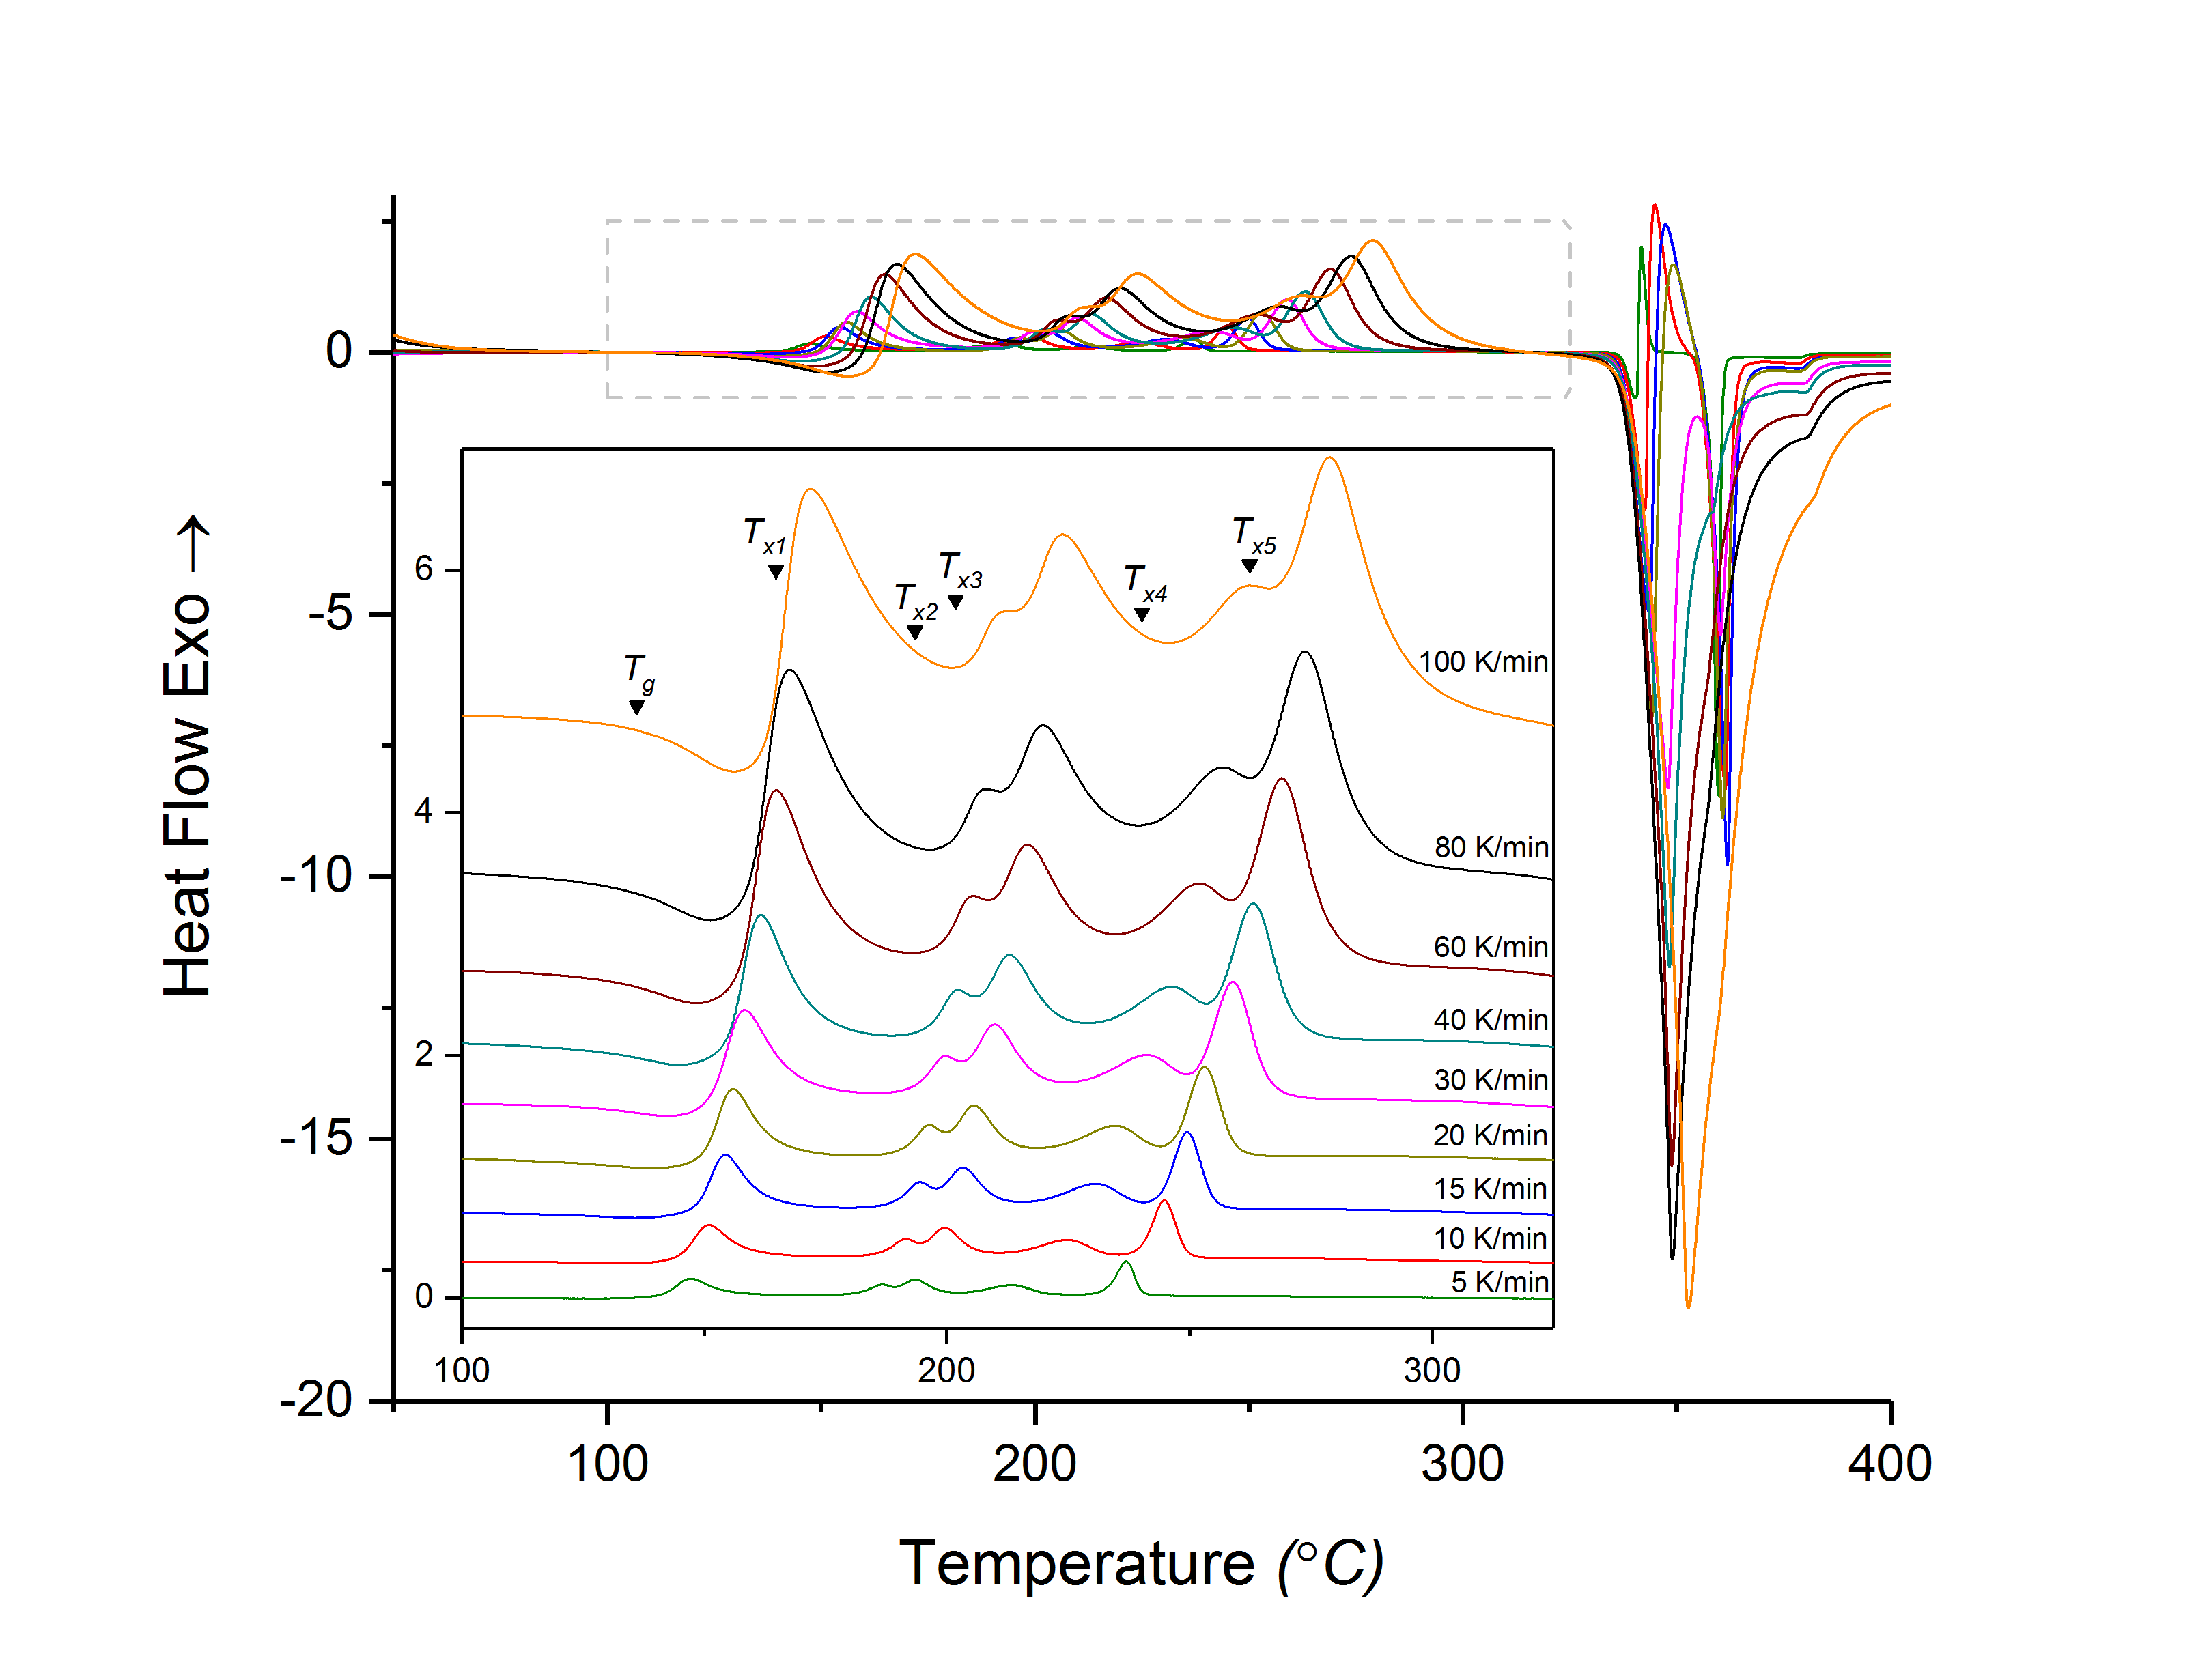
\includegraphics[width=\textwidth]{DSC_Fragility_Bulk.png}
		\caption{}
		\label{fig:DSC_vHeatingRate_Bulk}
	\end{subfigure}
	%Image 2
	\begin{subfigure}[htbp]{0.495\textwidth}
		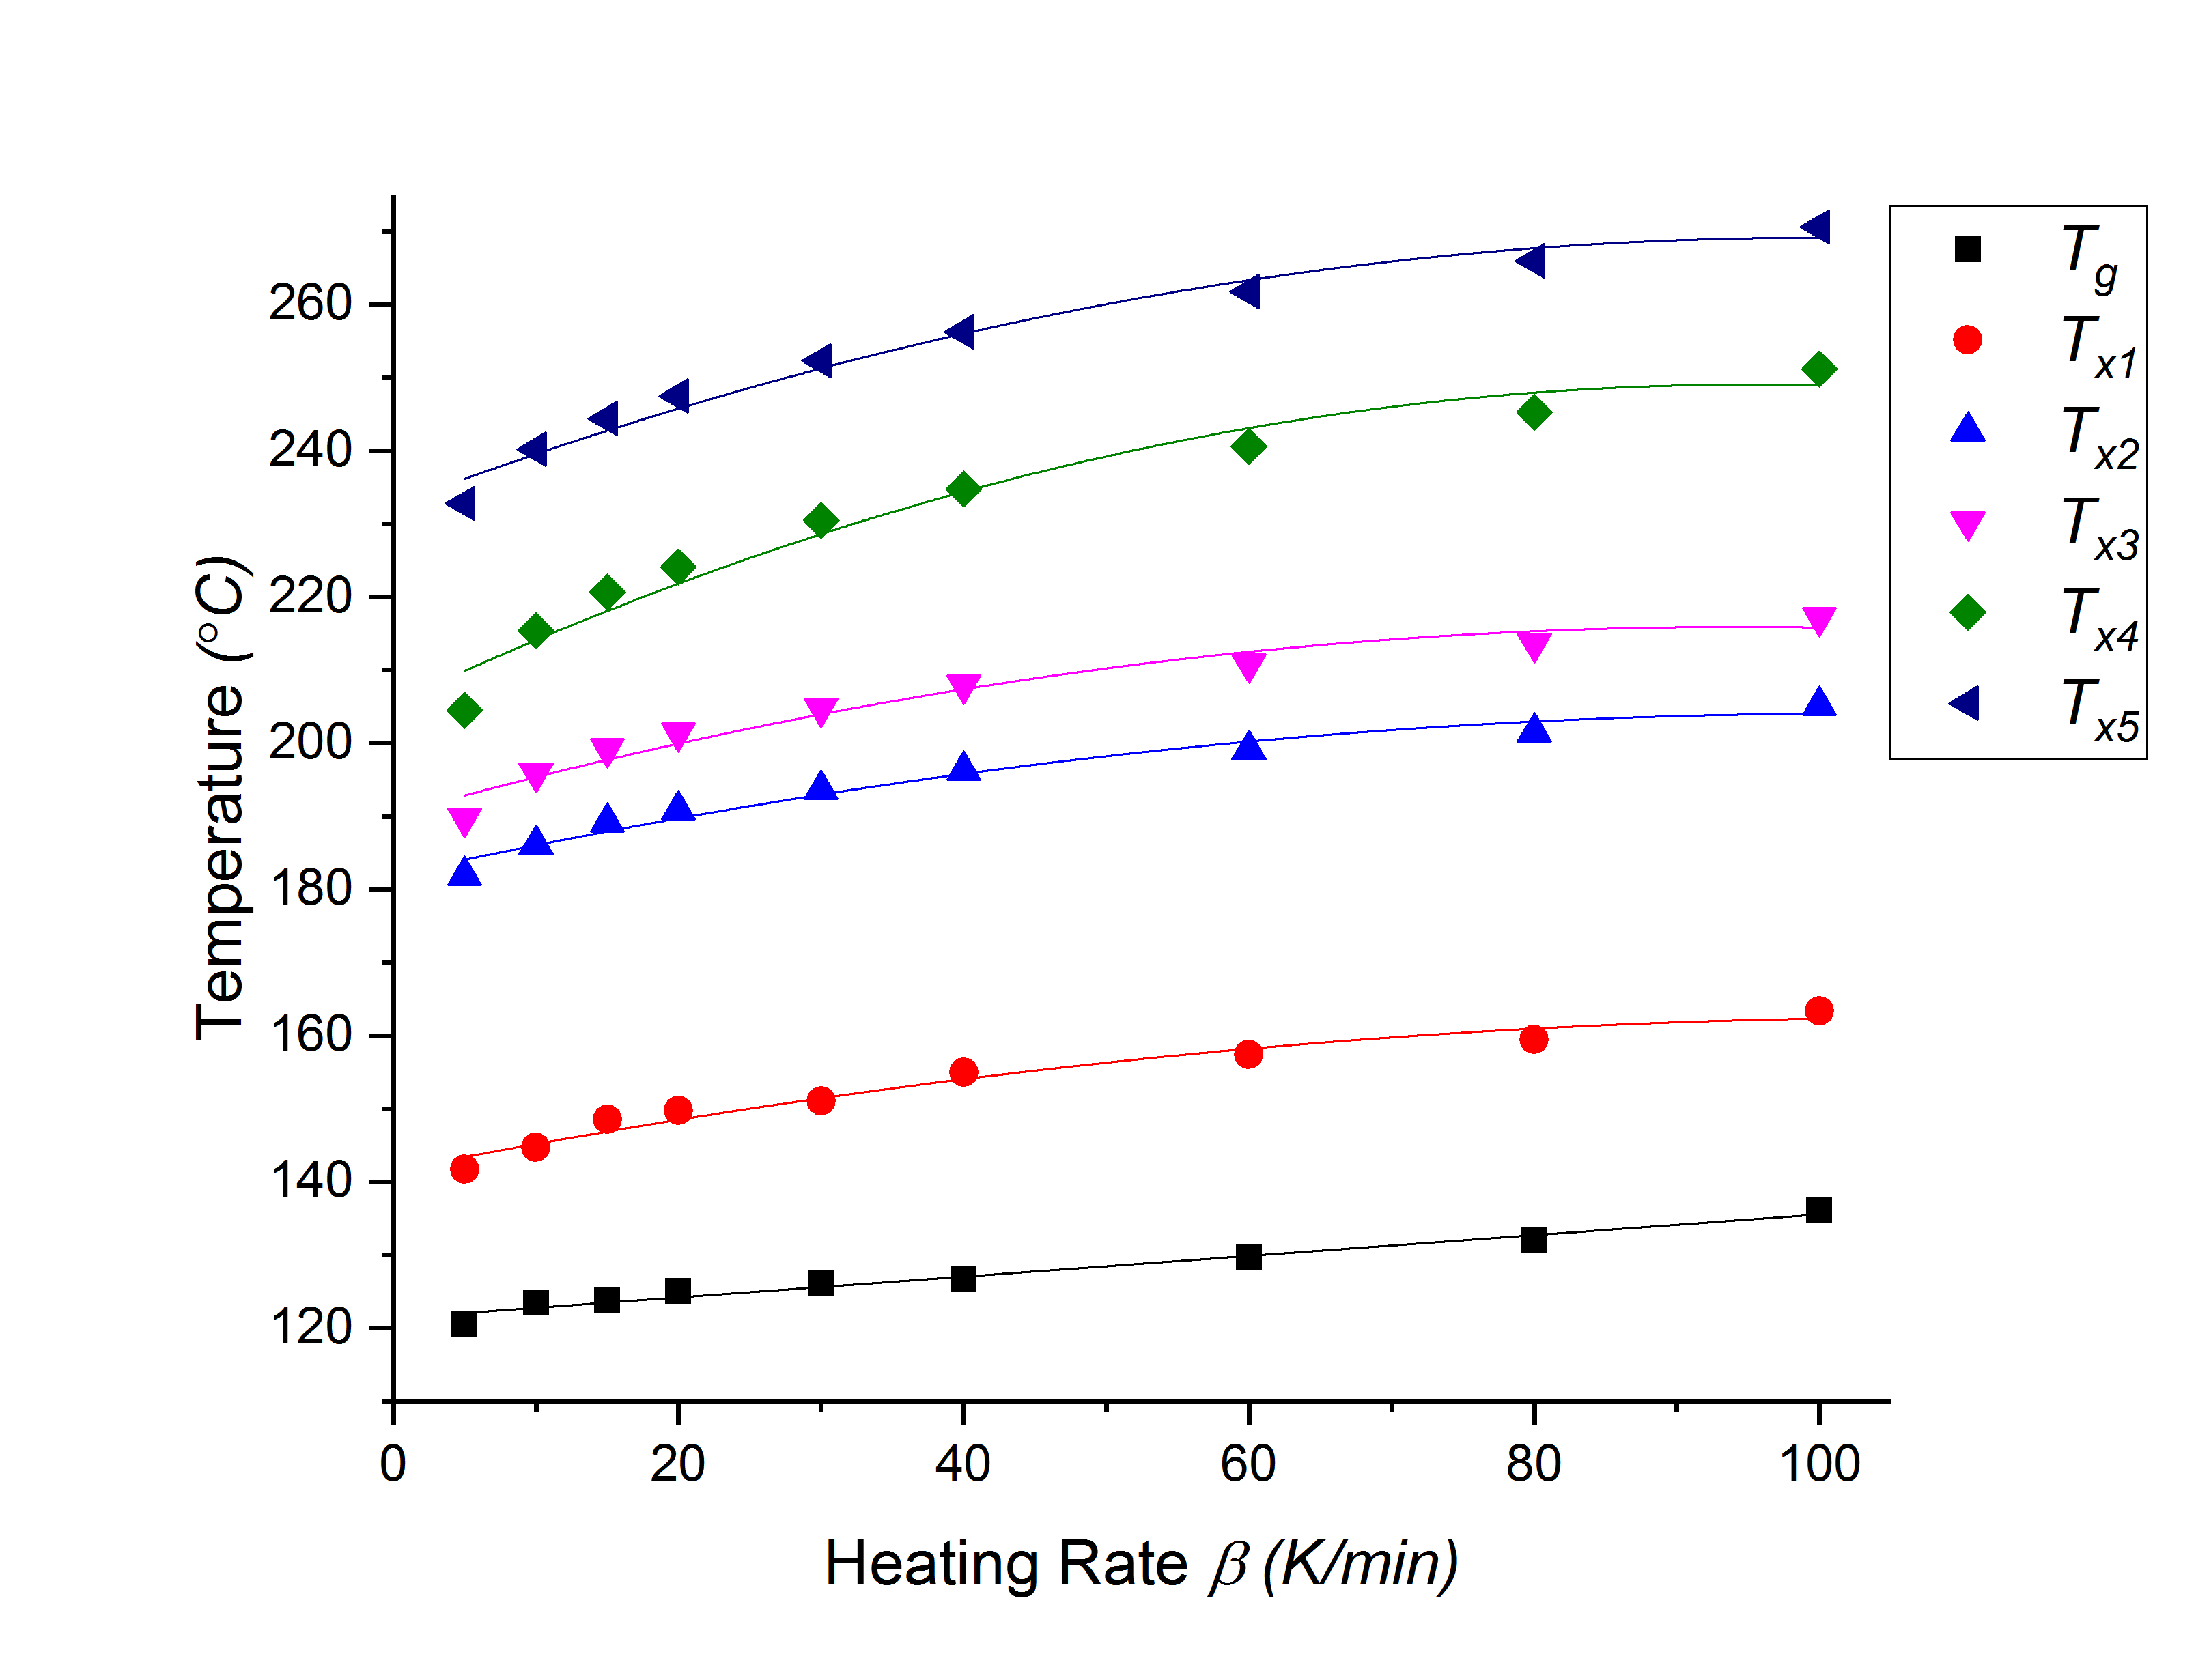
\includegraphics[width=\textwidth]{Bulk_Onset_Peaks_Relaxed_120C.png}
		\caption{}
		\label{fig:DSC_Onsets_Bulk}
	\end{subfigure}
	\caption{(a) Bulk \MgZnCa~ relaxed at 120 \degree C for 10 minutes and heated at various heating rates. The insert stacks the \gls{dsc} curves and labels the \Tg~ and \Tx es of the $100 K/min$ sample. (b) The \Tg s and \Tx es of the bulk \MgZnCa~ at all heating rates. }%global caption
	\label{fig:DSC_Bulk}
\end{figure}

%code to put 2 images side by side in a figure
\begin{figure}[b]
	\centering
	%Image 1
	\begin{subfigure}[htbp]{0.495\textwidth}
		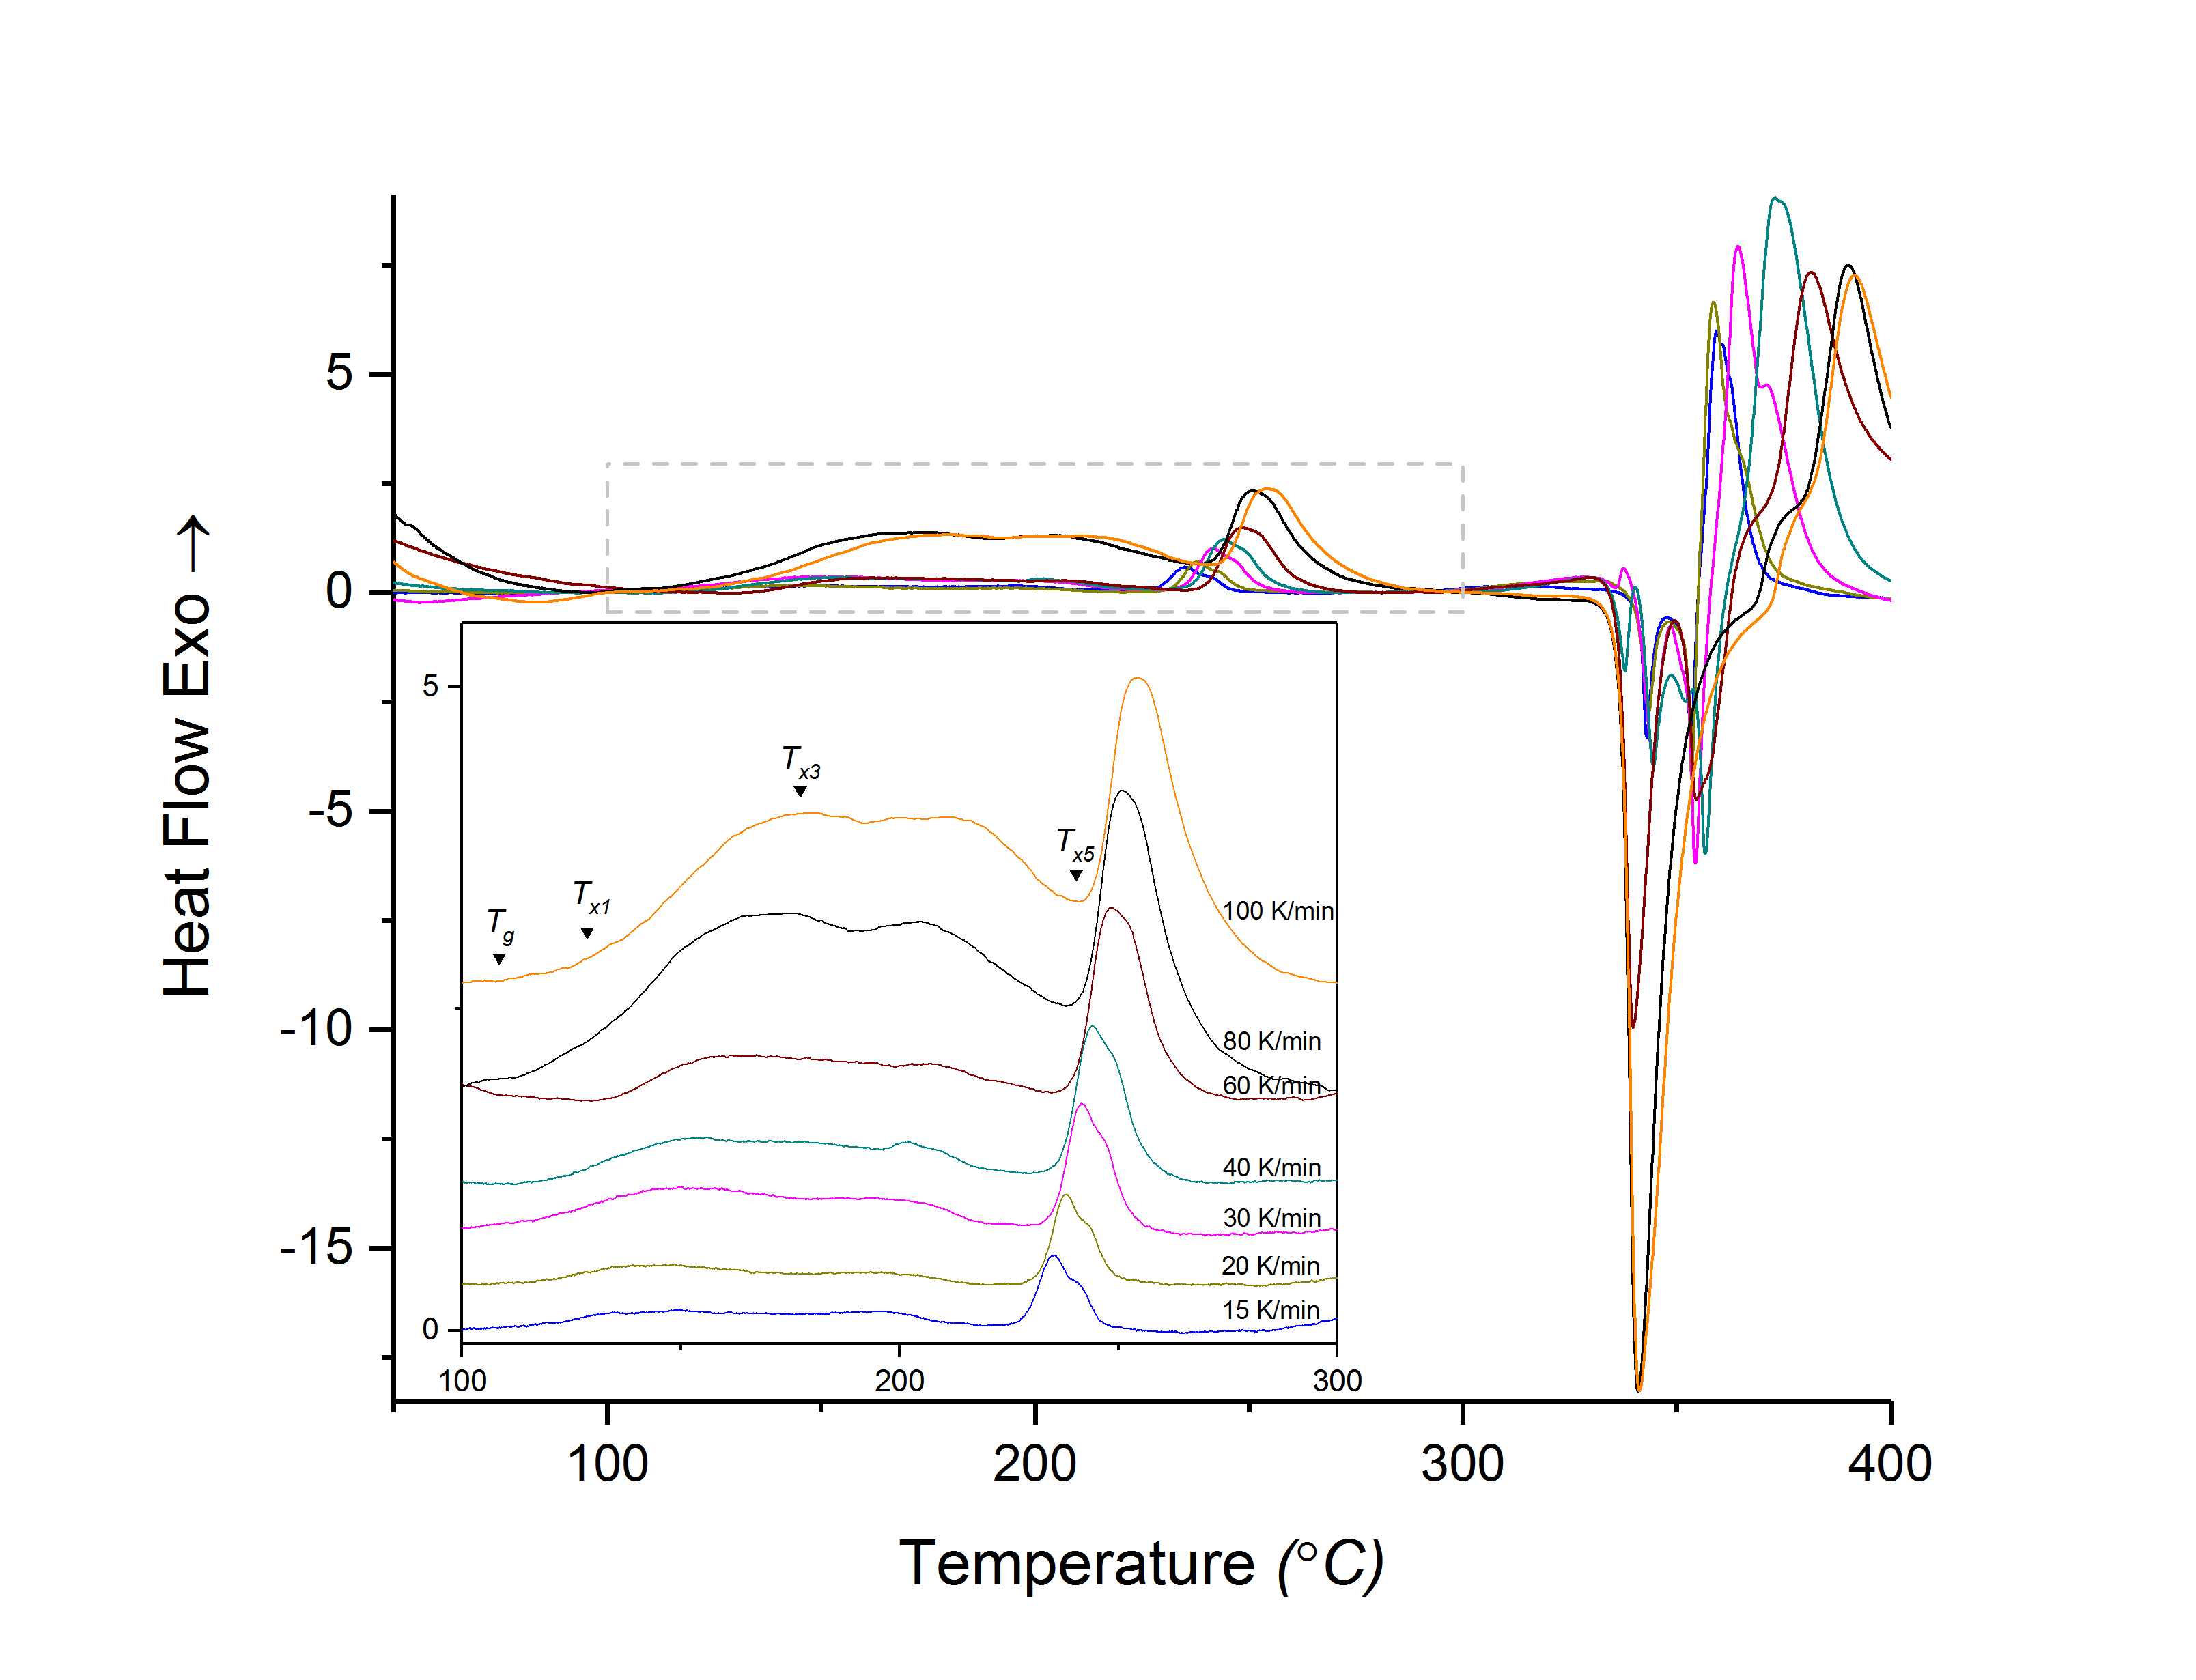
\includegraphics[width=\textwidth]{DSC_Fragility_Film.png}
		\caption{}
		\label{fig:DSC_vHeatingRate_Film}
	\end{subfigure}
	%Image 2
	\begin{subfigure}[htbp]{0.495\textwidth}
		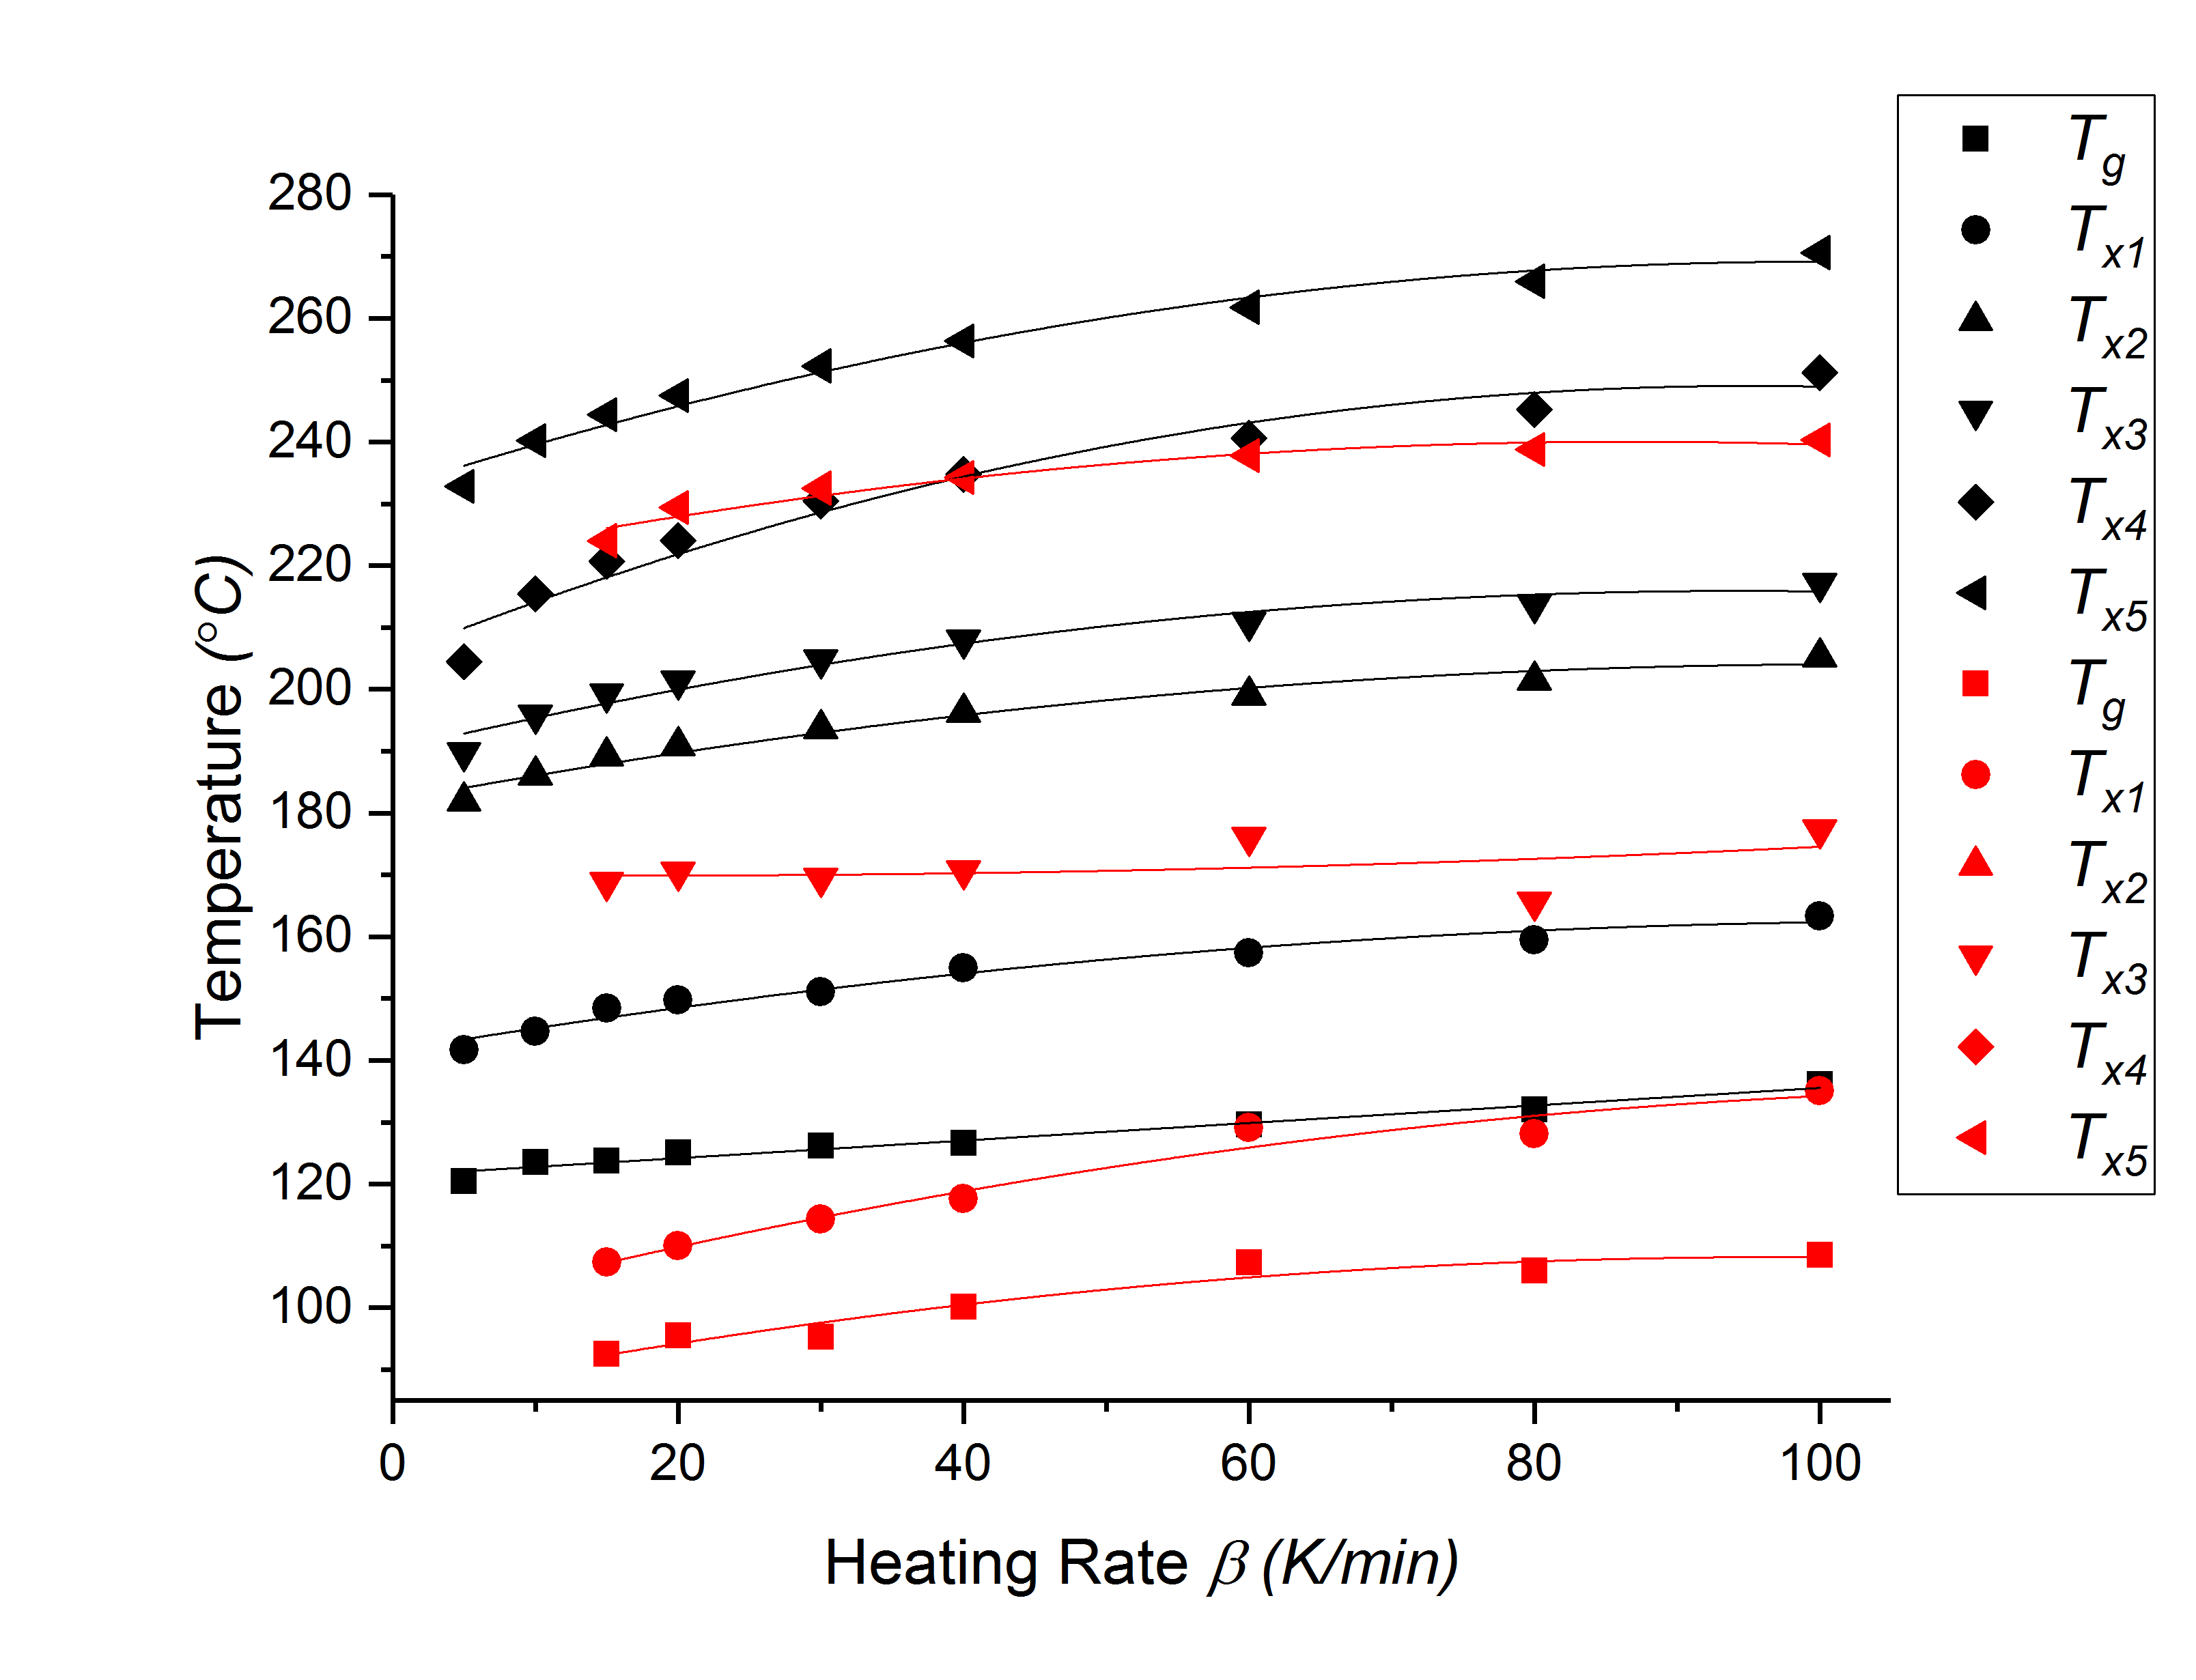
\includegraphics[width=\textwidth]{Onsets_BulkandFilm.png}
		\caption{}
		\label{fig:DSC_Onsets_Film}
	\end{subfigure}
	\caption{(a) Unrelaxed film \MgZnCa~ heated at various heating rates. The insert stacks the \gls{dsc} curves and labels the \Tg~ and \Tx es of the $100 K/min$ sample. (b) The \Tg s and \Tx es of the bulk and film \MgZnCa~ at all heating rates. }%global caption
	\label{fig:DSC_Film}
\end{figure}

%single image
\begin{figure}[b]
	\centering
	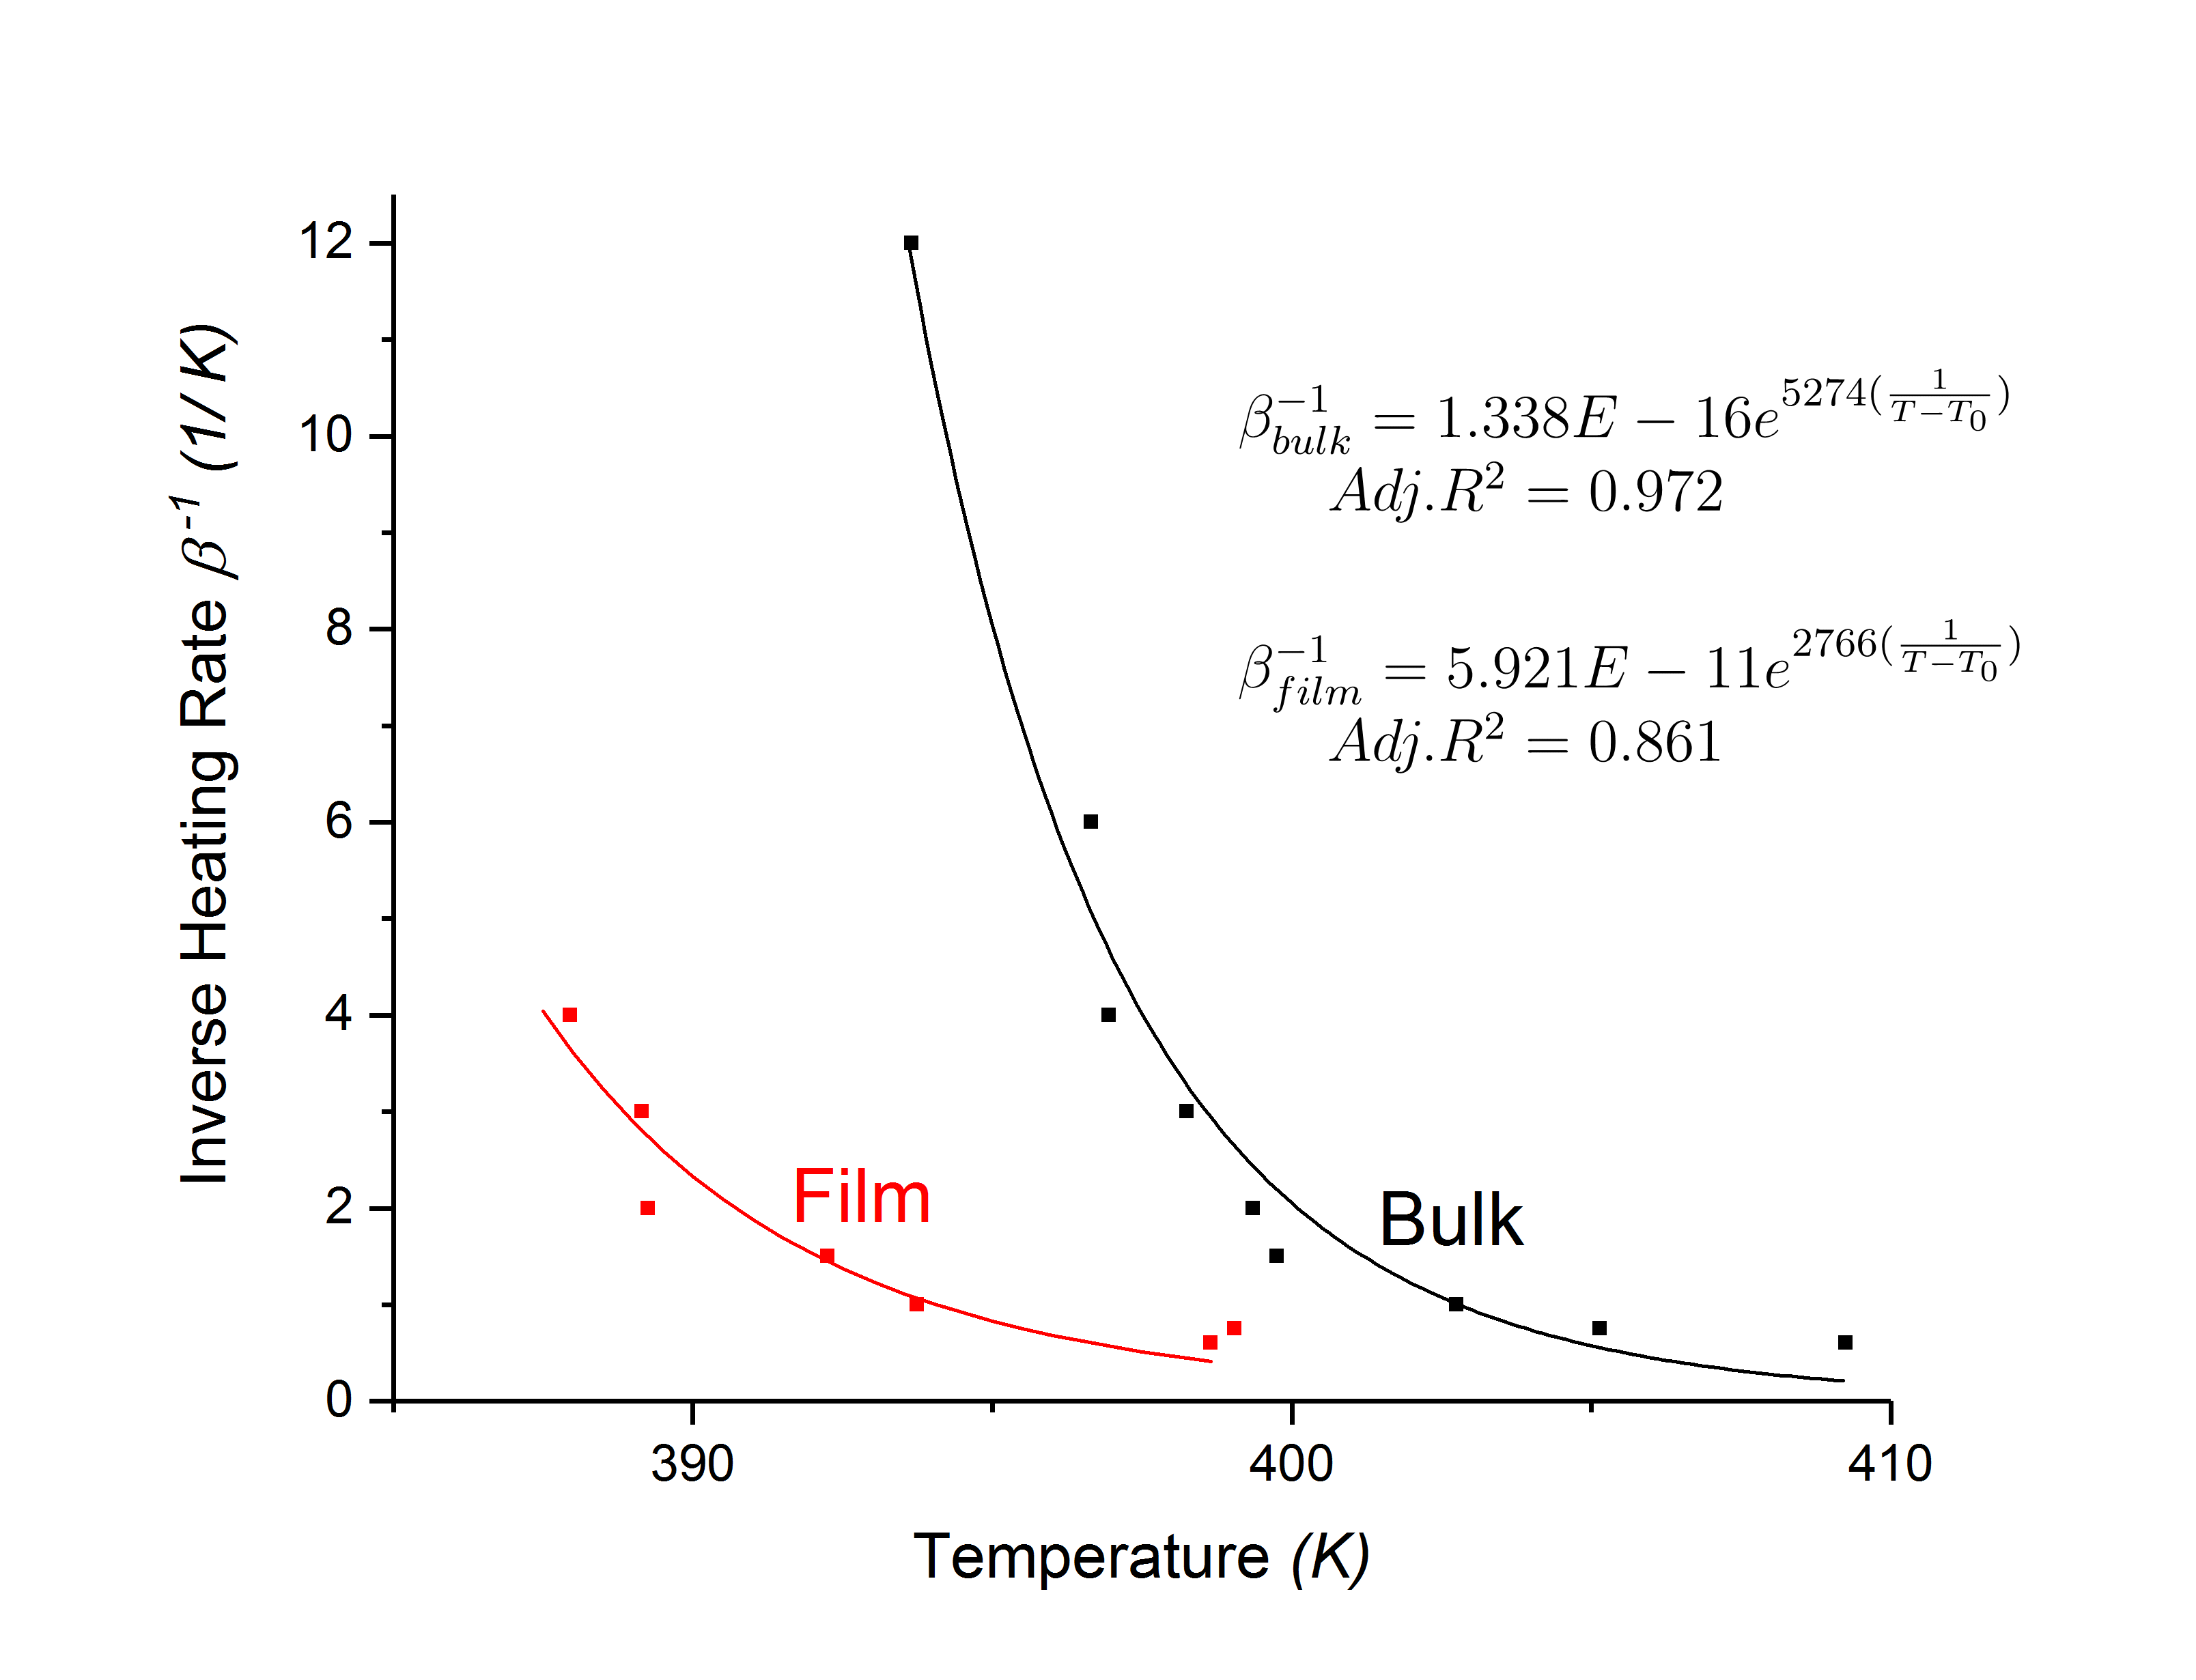
\includegraphics[width=0.95\textwidth]{Bulk_Film_Fragility.png}
	\caption[Table of contents Capition]{Fitted fragility for the \MgZnCa system obtained by \acrshort{dsc} at various heating rates}
	\label{fig:Fragility_BulkFilm_mValue}
\end{figure}

%single image
\begin{figure}[b]
	\centering
	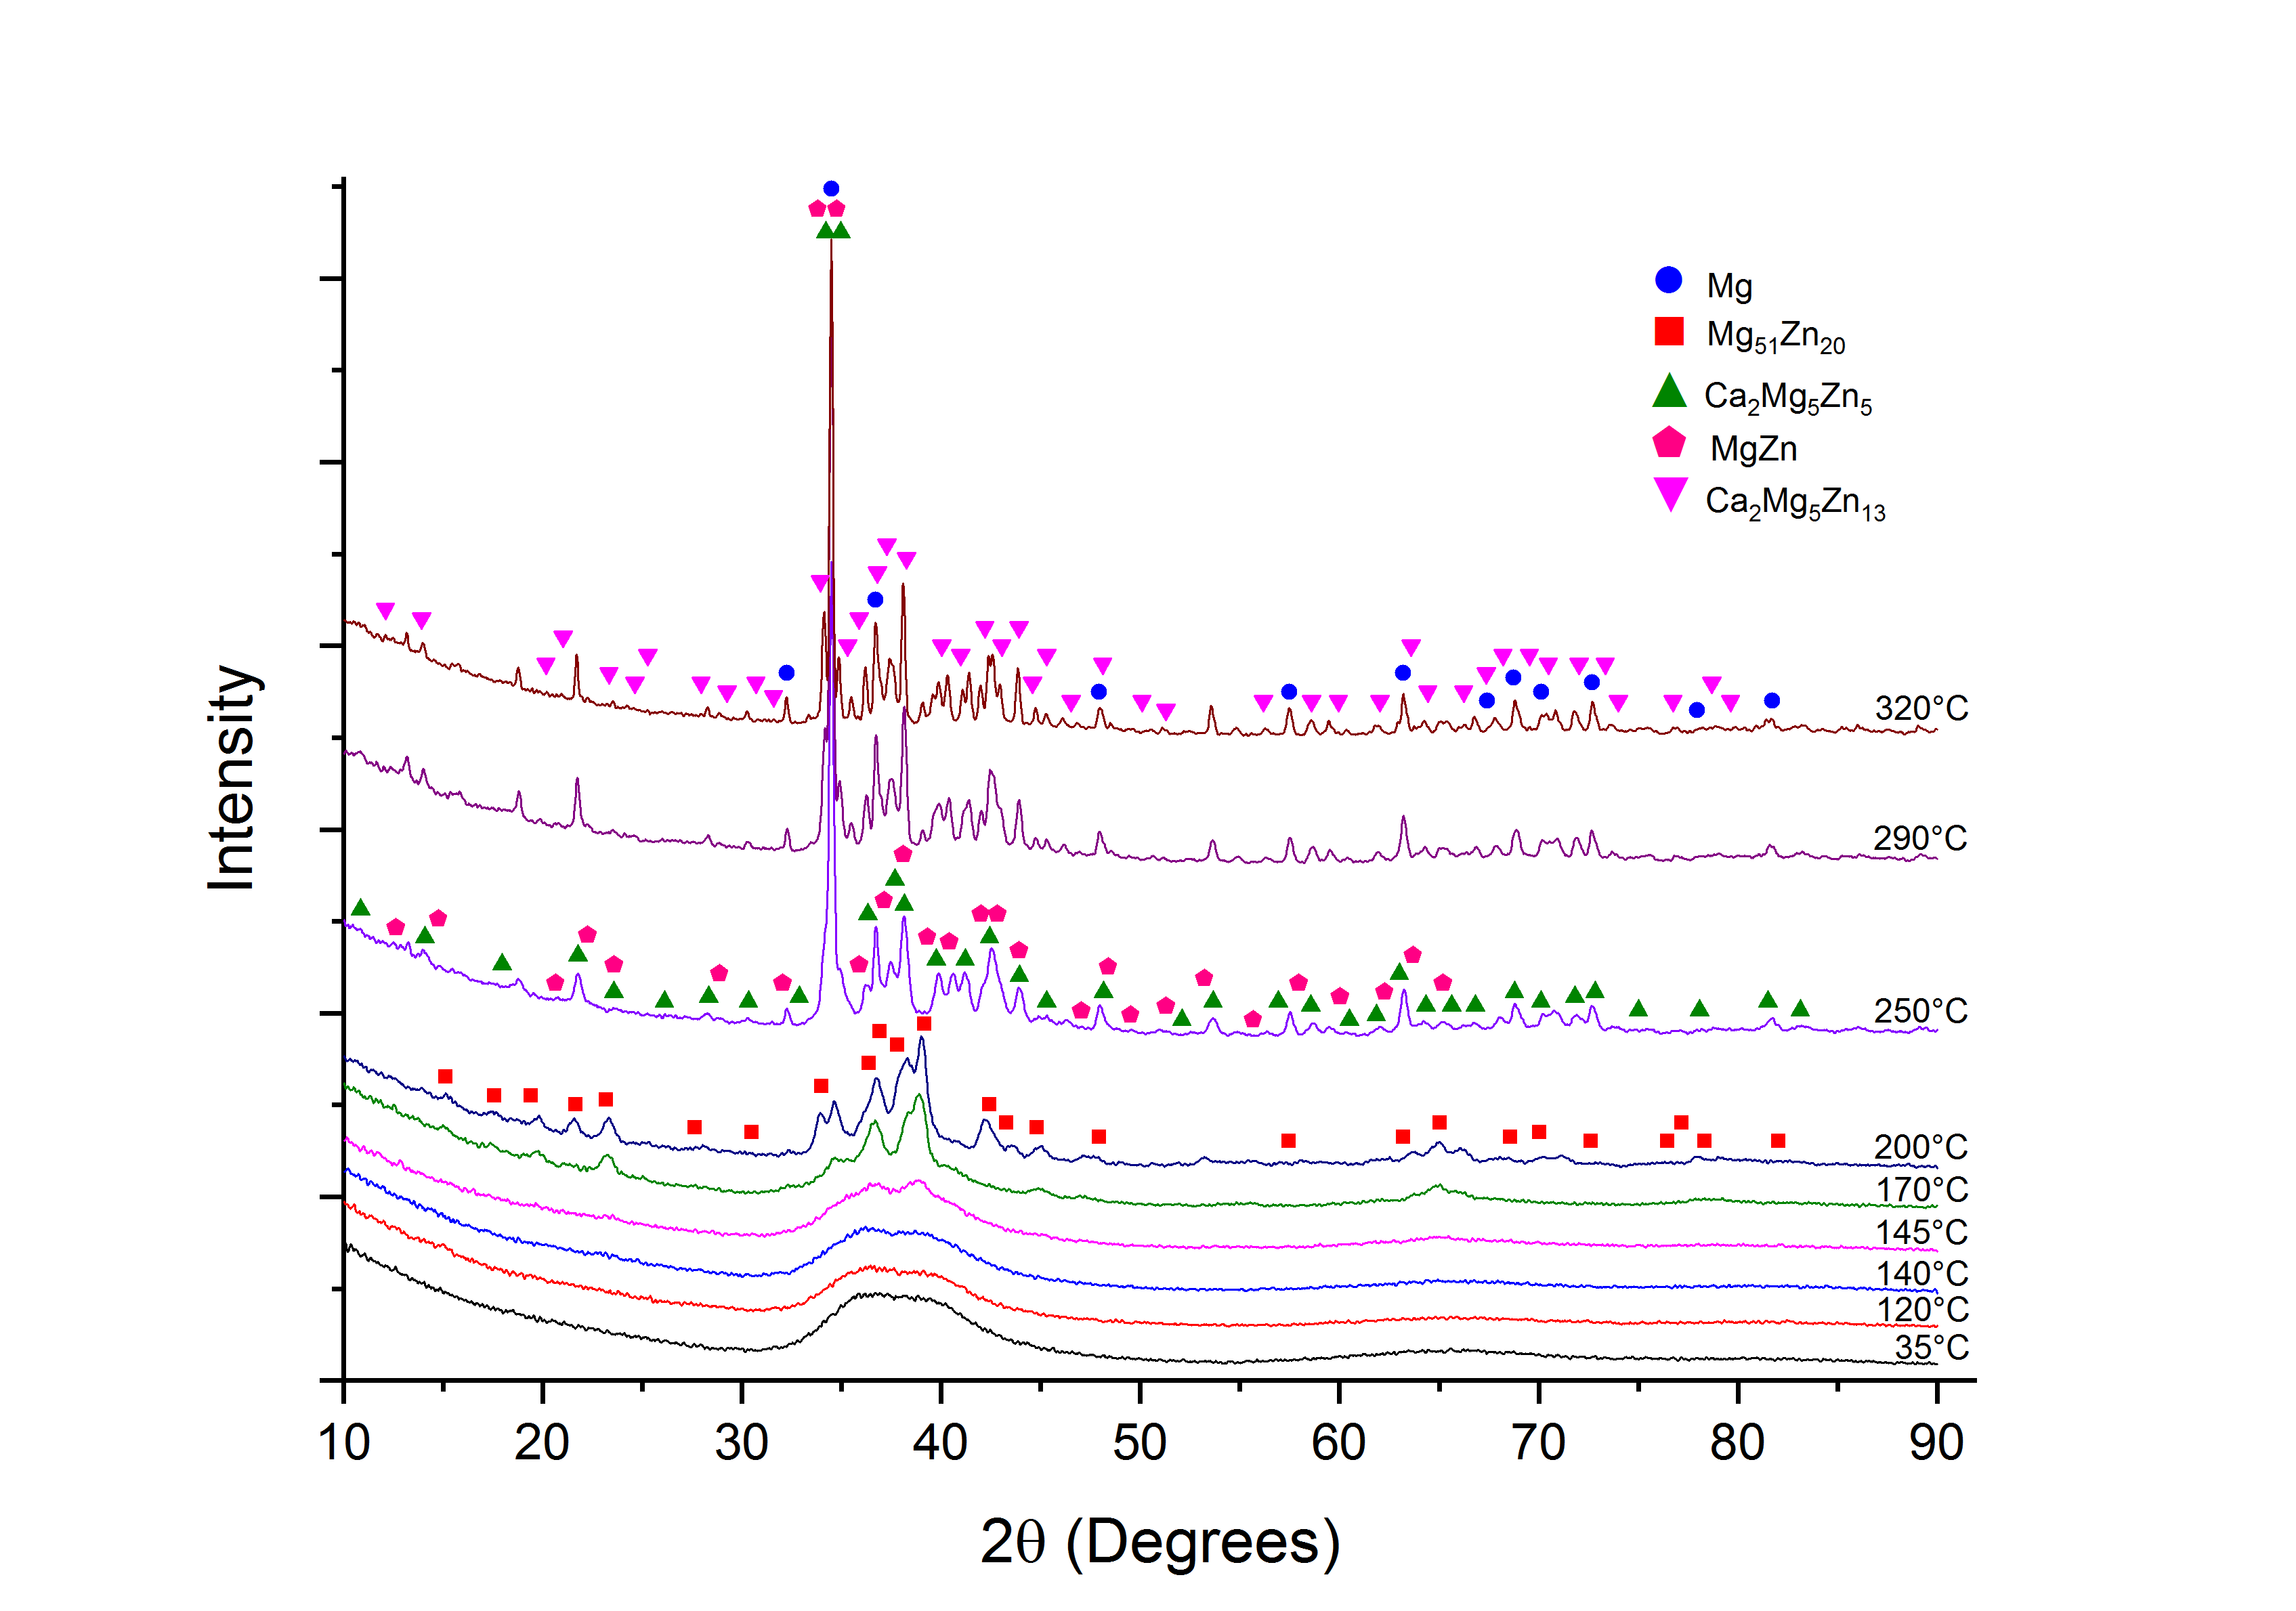
\includegraphics[width=0.9\textwidth]{XRD_Annealing_Bulk.png}
	\caption[Table of contents Capition]{\acrshort{xrd} pattern for Bulk \MgZnCa~ heated through several crystallization peaks identified from \acrshort{dsc}}
	\label{fig:XRD_Annealing_Bulk}
\end{figure}

%single image
\begin{figure}[b]
	\centering
	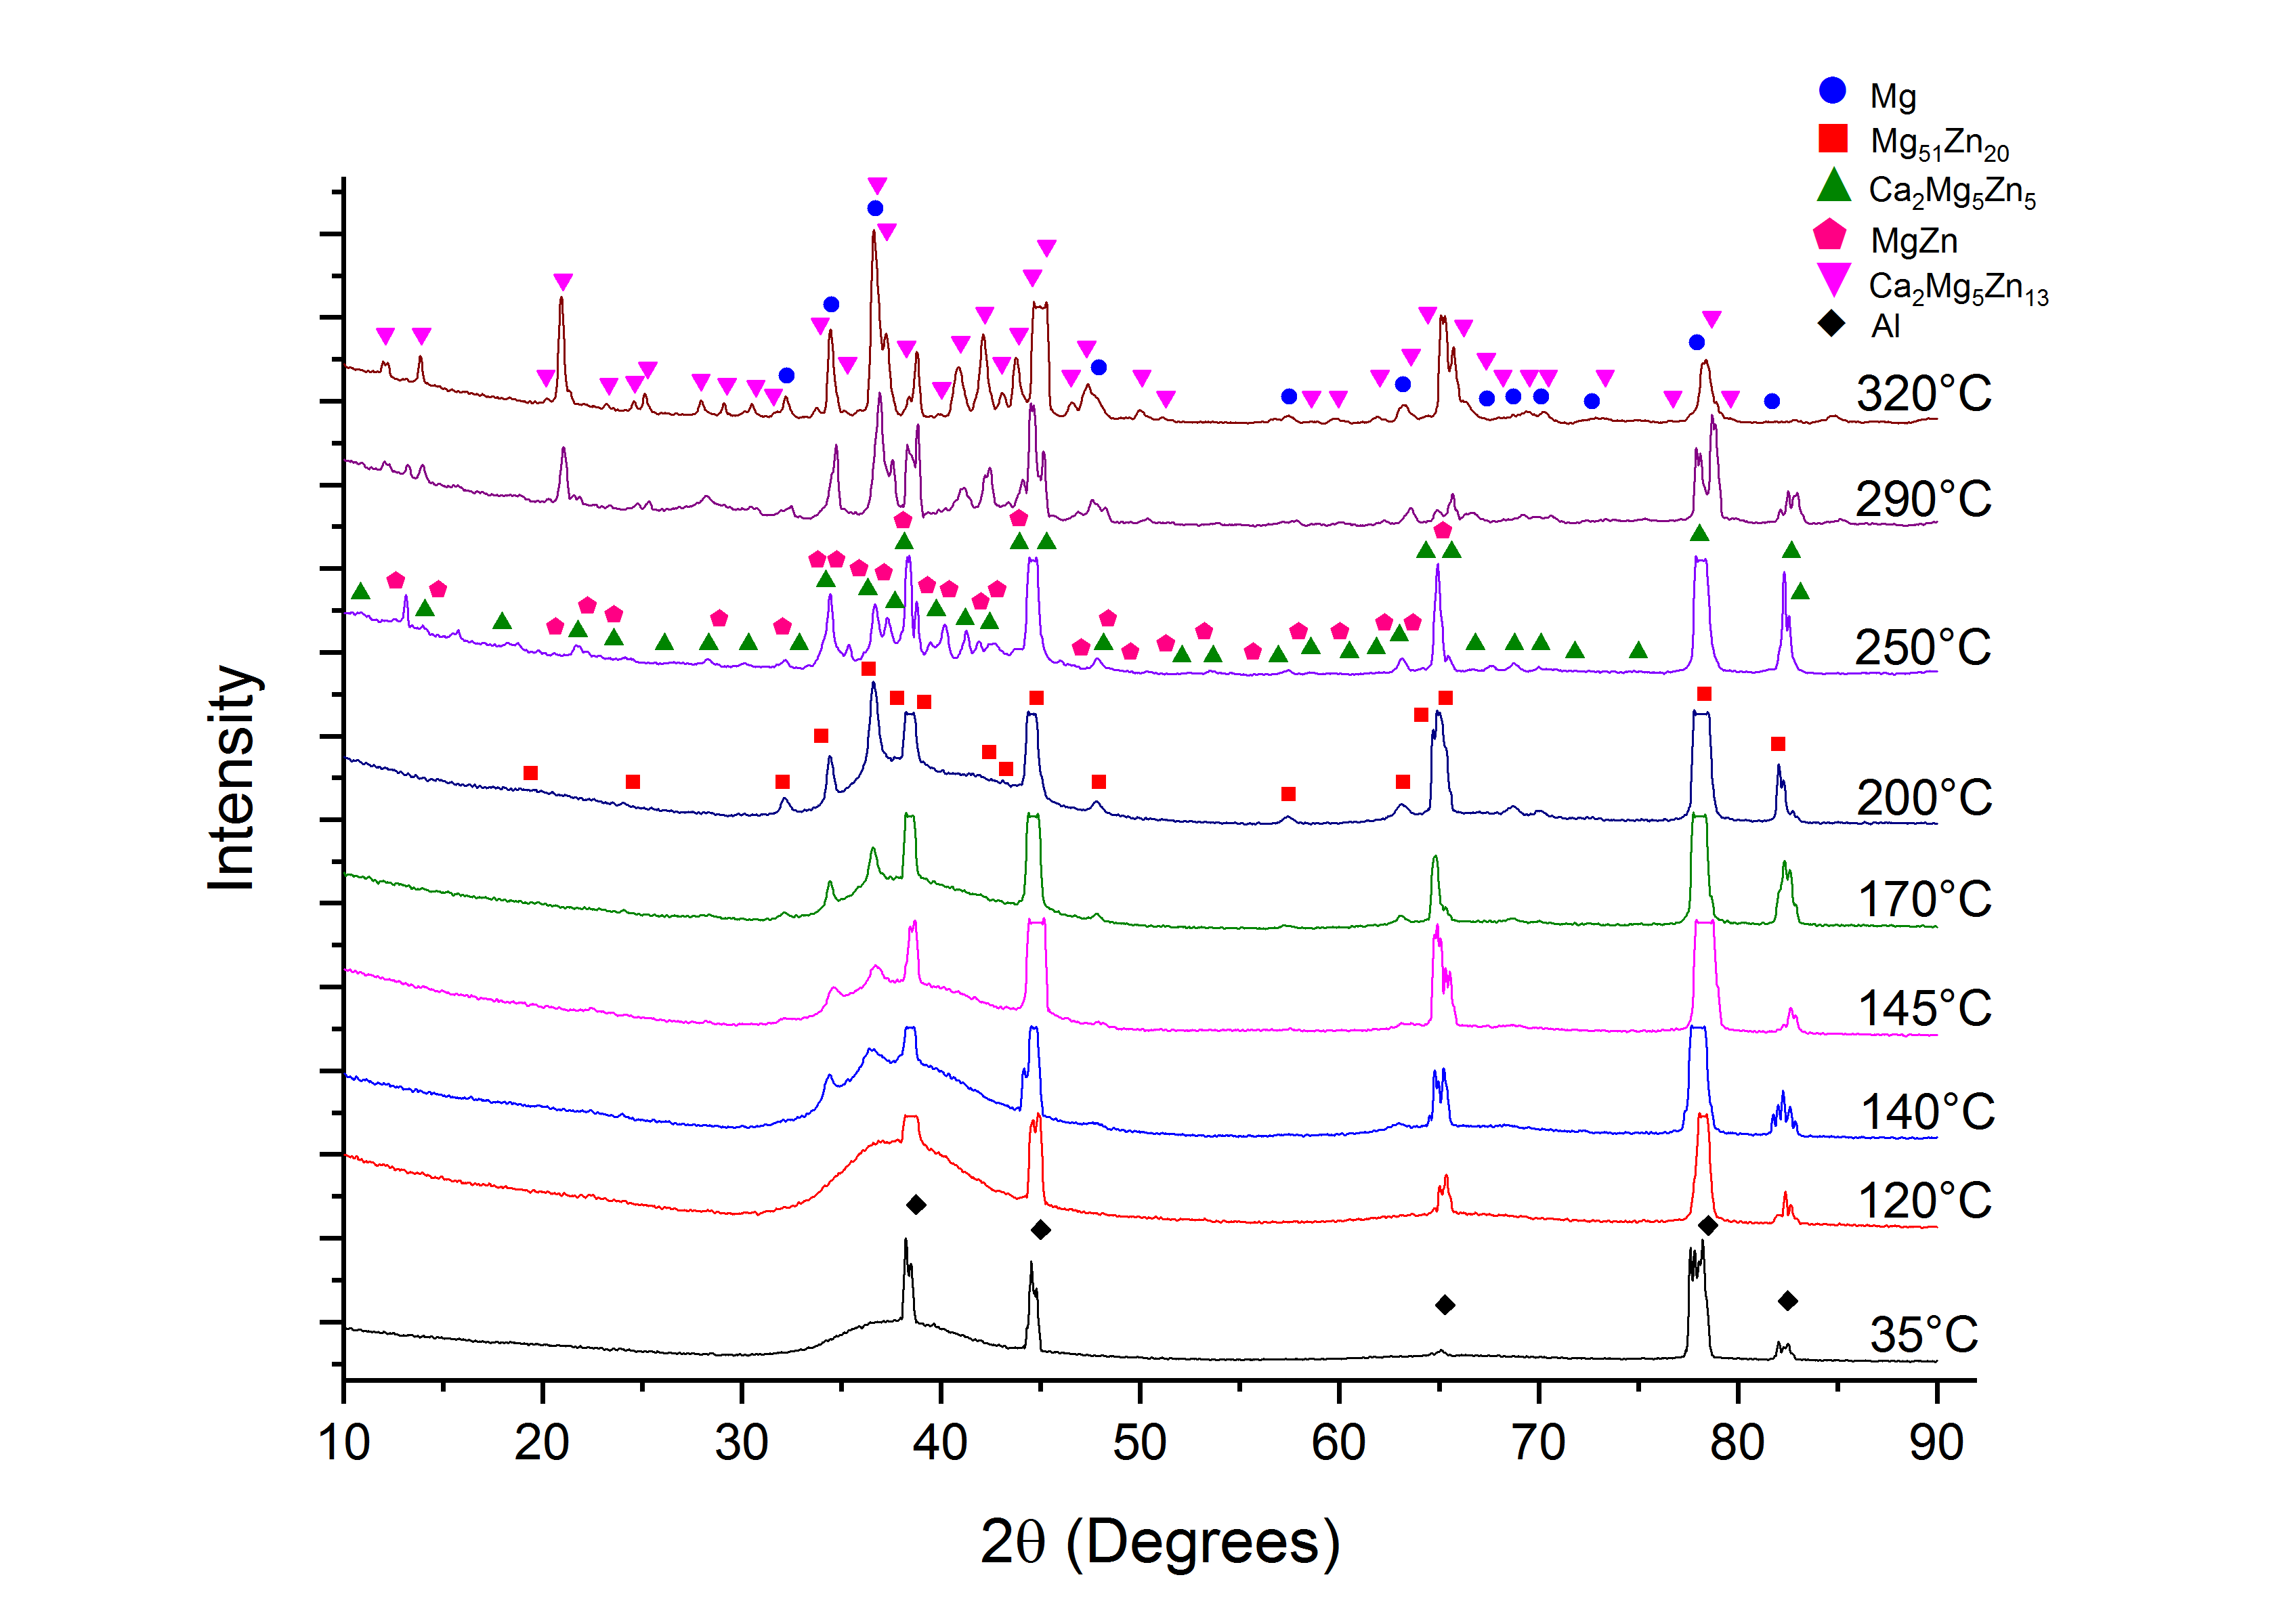
\includegraphics[width=0.9\textwidth]{XRD_Annealing_Film.png}
	\caption[Table of contents Capition]{\acrshort{xrd} pattern for Film \MgZnCa~ heated through several crystallization peaks identified from \acrshort{dsc}}
	\label{fig:XRD_Annealing_Film}
\end{figure}

%code to put 2 images side by side in a figure
\begin{figure}[b]
	\centering
	%Image 1
	\begin{subfigure}[htbp]{0.75\textwidth}
		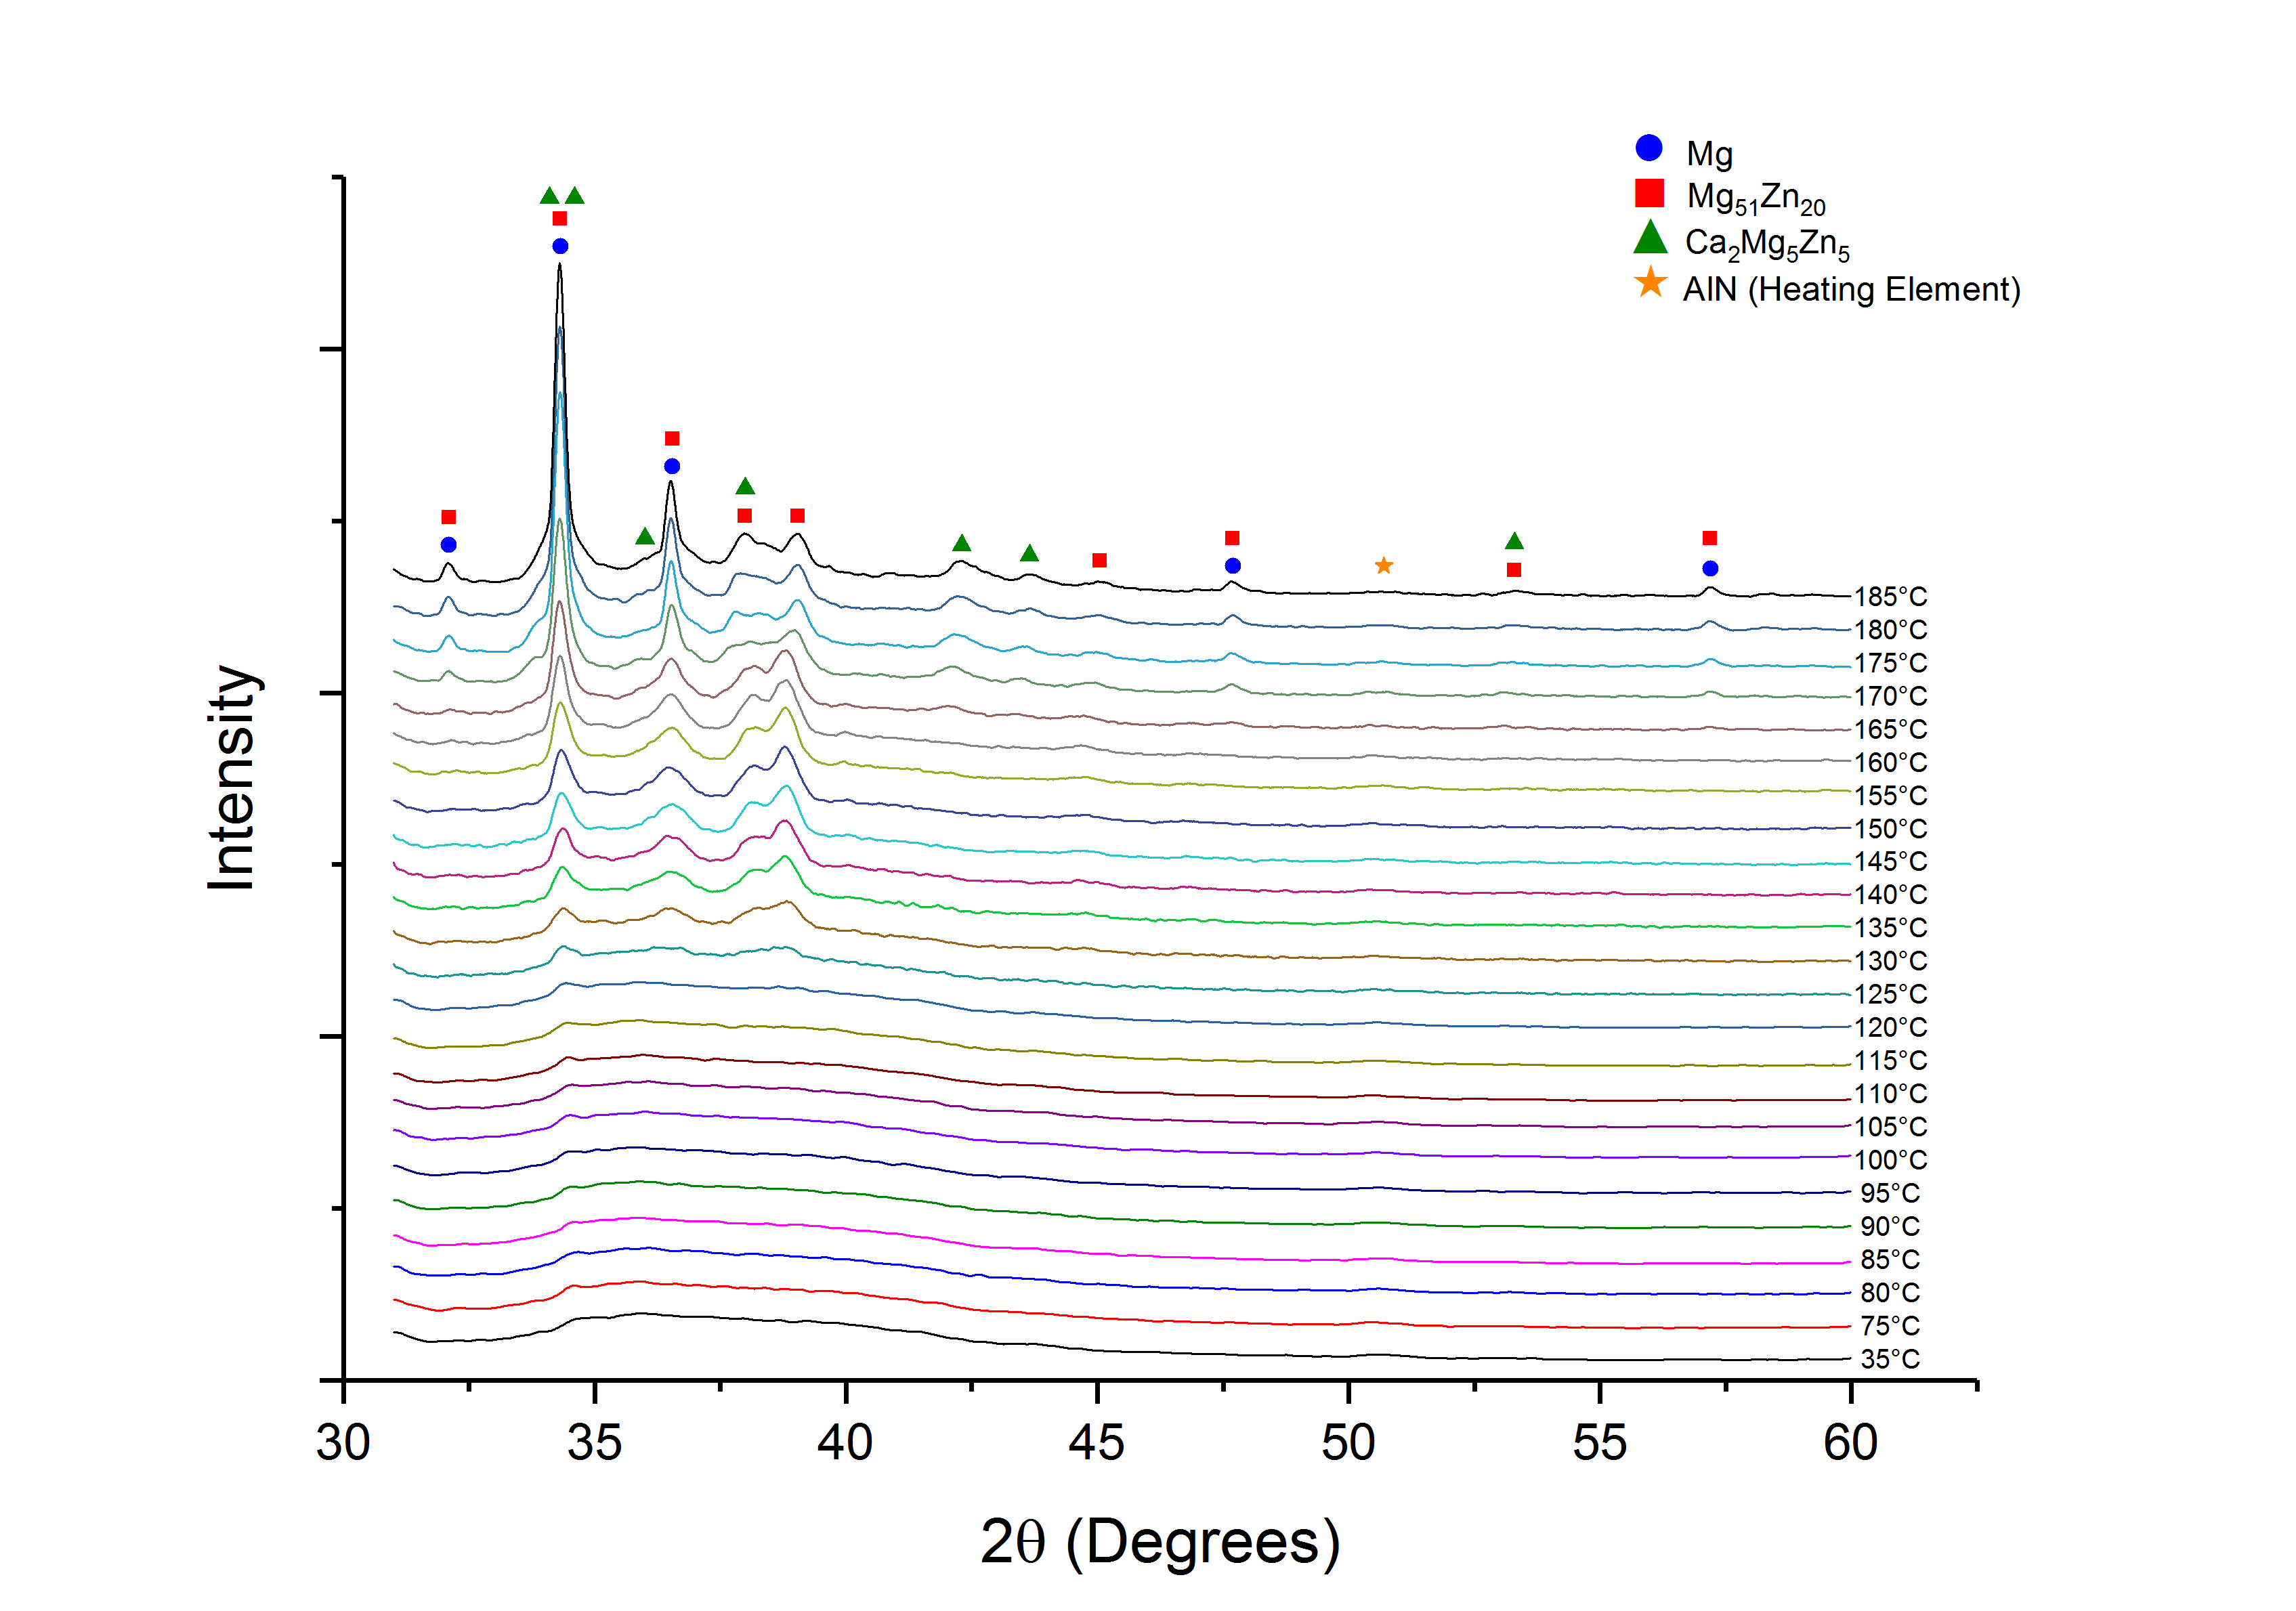
\includegraphics[width=\textwidth]{XRD_Dynamic_Bulk.png}
		\caption{}
		\label{fig:XRD_Dynamic_FullStack_Bulk}
	\end{subfigure}
	%Image 2
	\begin{subfigure}[htbp]{0.75\textwidth}
		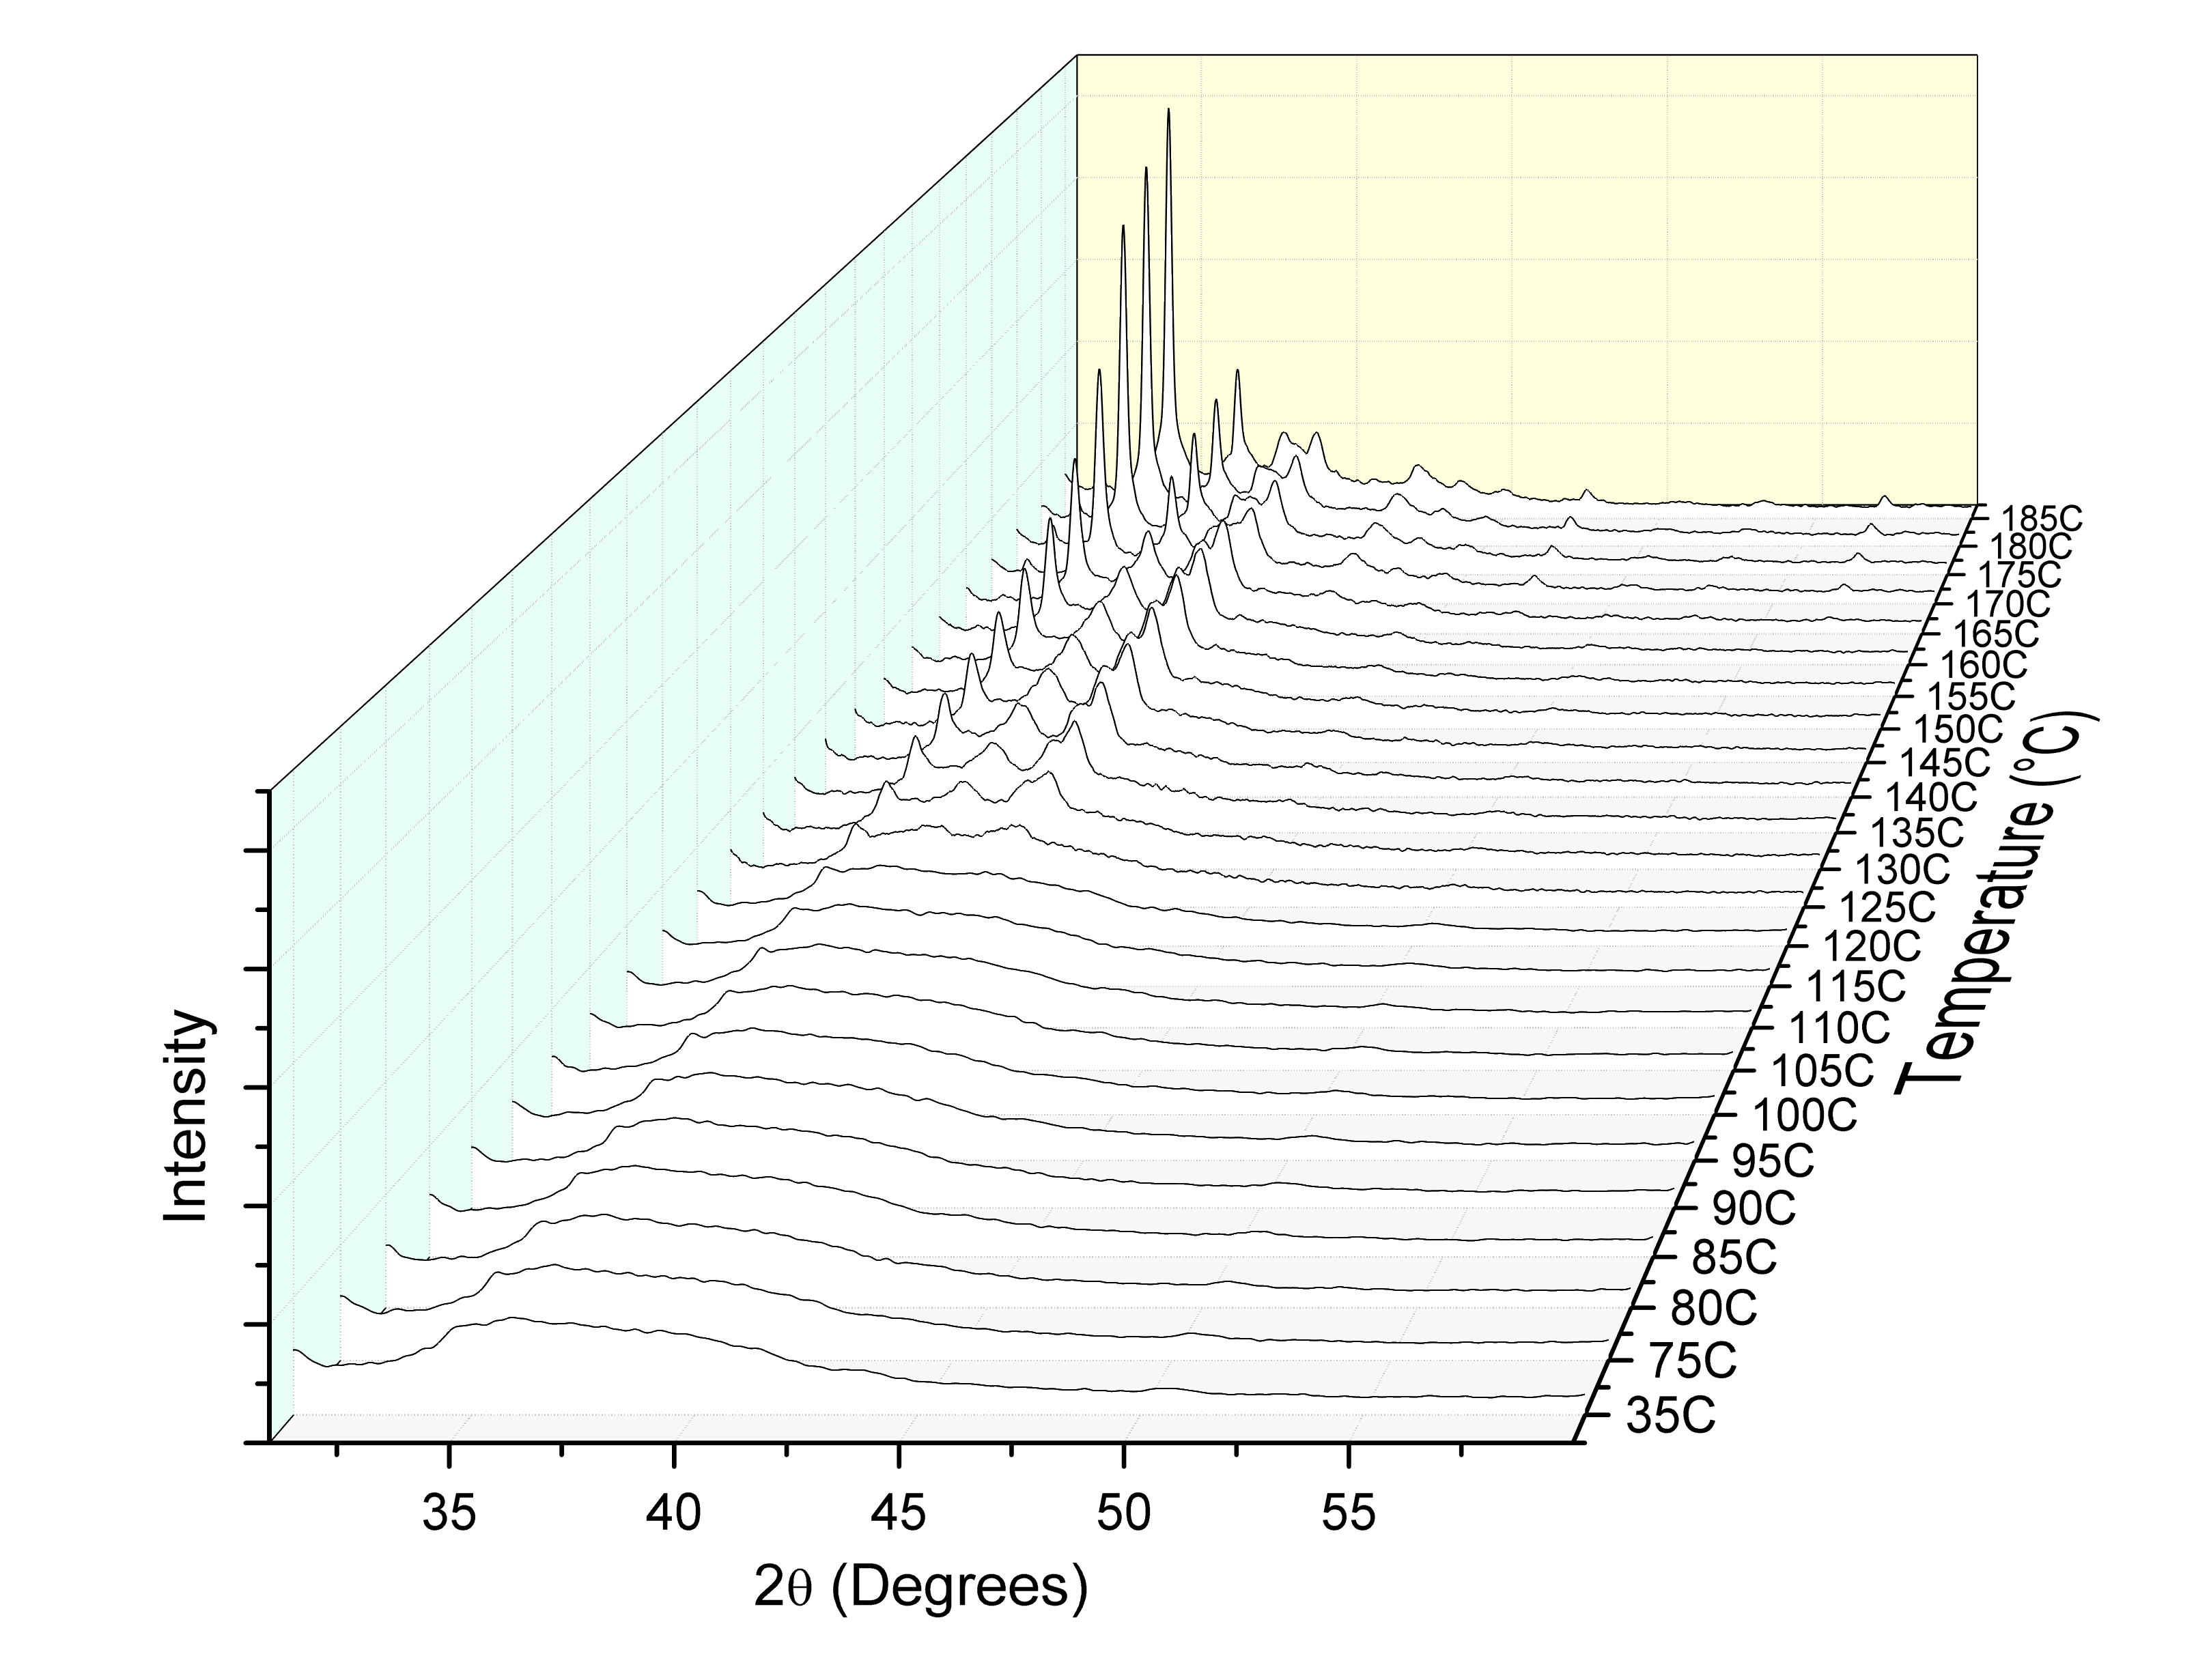
\includegraphics[width=\textwidth]{Bulk_Heated_XRD_Waterfall3D_Smooth2.png}
		\caption{}
		\label{fig:XRD_Dynamic_WaterFall_Bulk}
	\end{subfigure}
	\caption{(a) Stacked \gls{xrd} patterns from the incremental heating of bulk \MgZnCa. (b) Cascading \gls{xrd} patterns from the incremental heating of bulk \MgZnCa. }%global caption
	\label{fig:XRD_Dynamic_Bulk}
\end{figure}

%code to put 2 images side by side in a figure
\begin{figure}[b]
	\centering
	%Image 1
	\begin{subfigure}[htbp]{0.75\textwidth}
		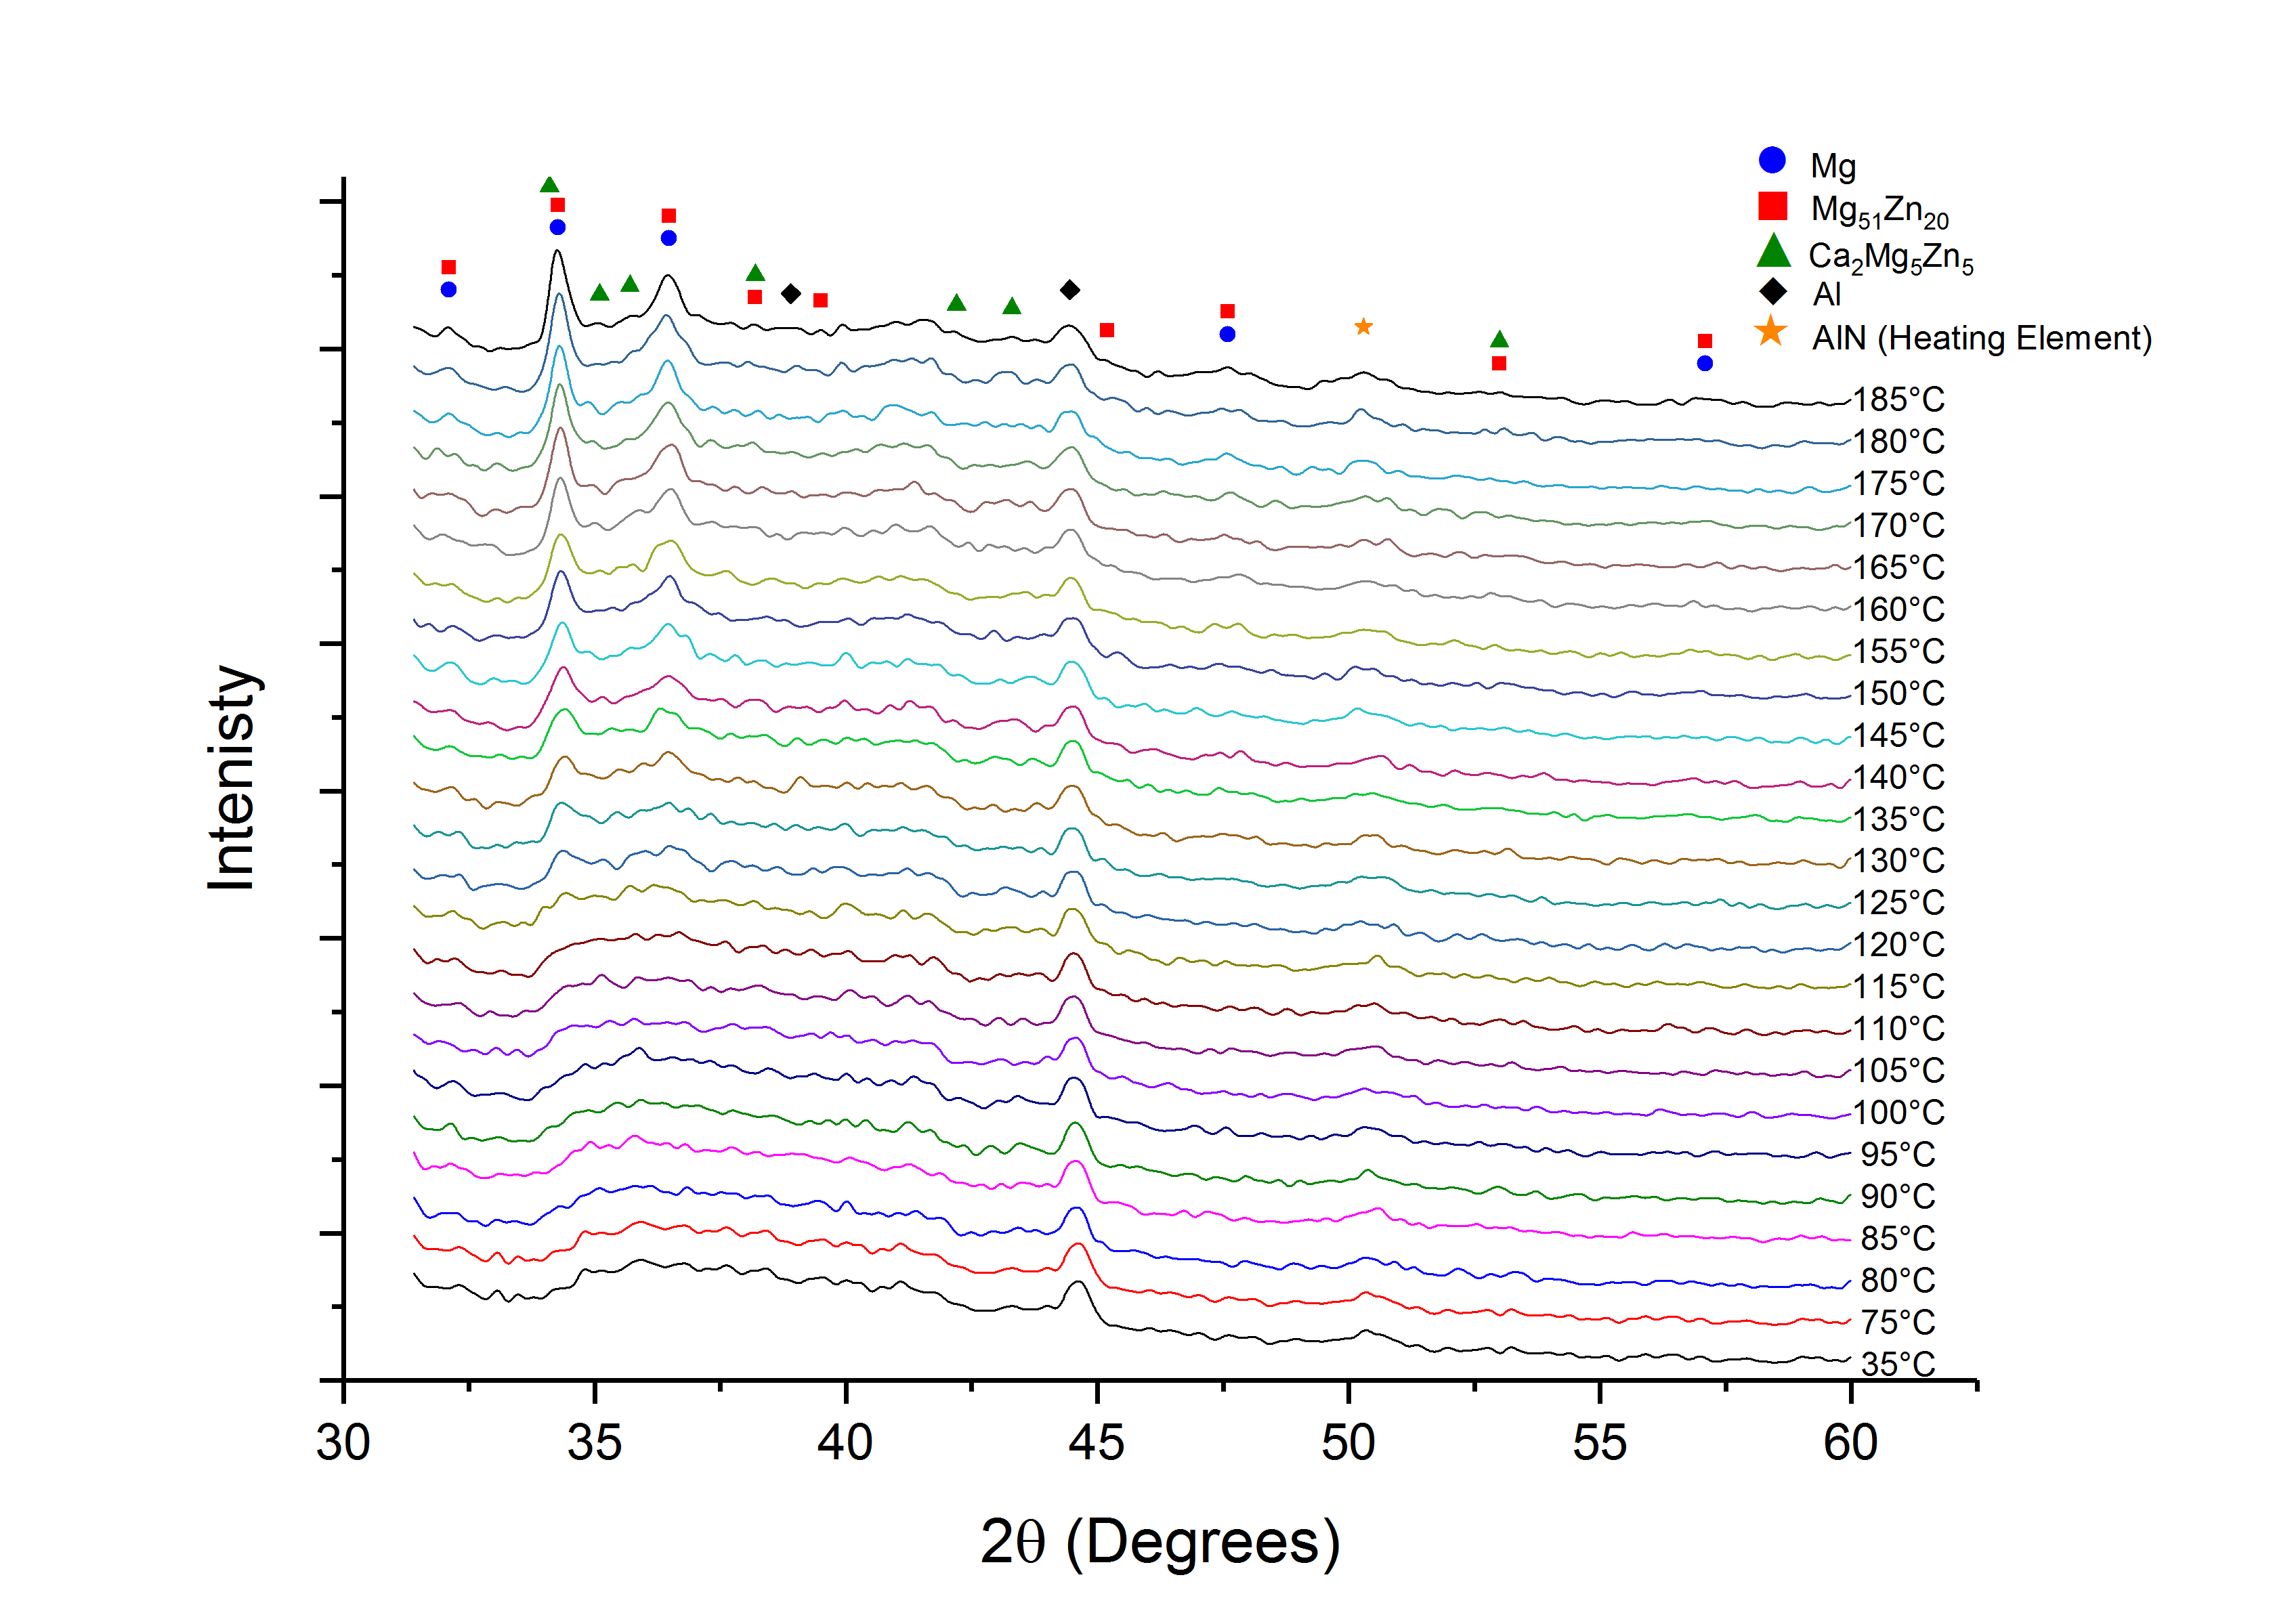
\includegraphics[width=\textwidth]{XRD_Dynamic_Film.png}
		\caption{}
		\label{fig:XRD_Dynamic_FullStack_Film}
	\end{subfigure}
	%Image 2
	\begin{subfigure}[htbp]{0.75\textwidth}
		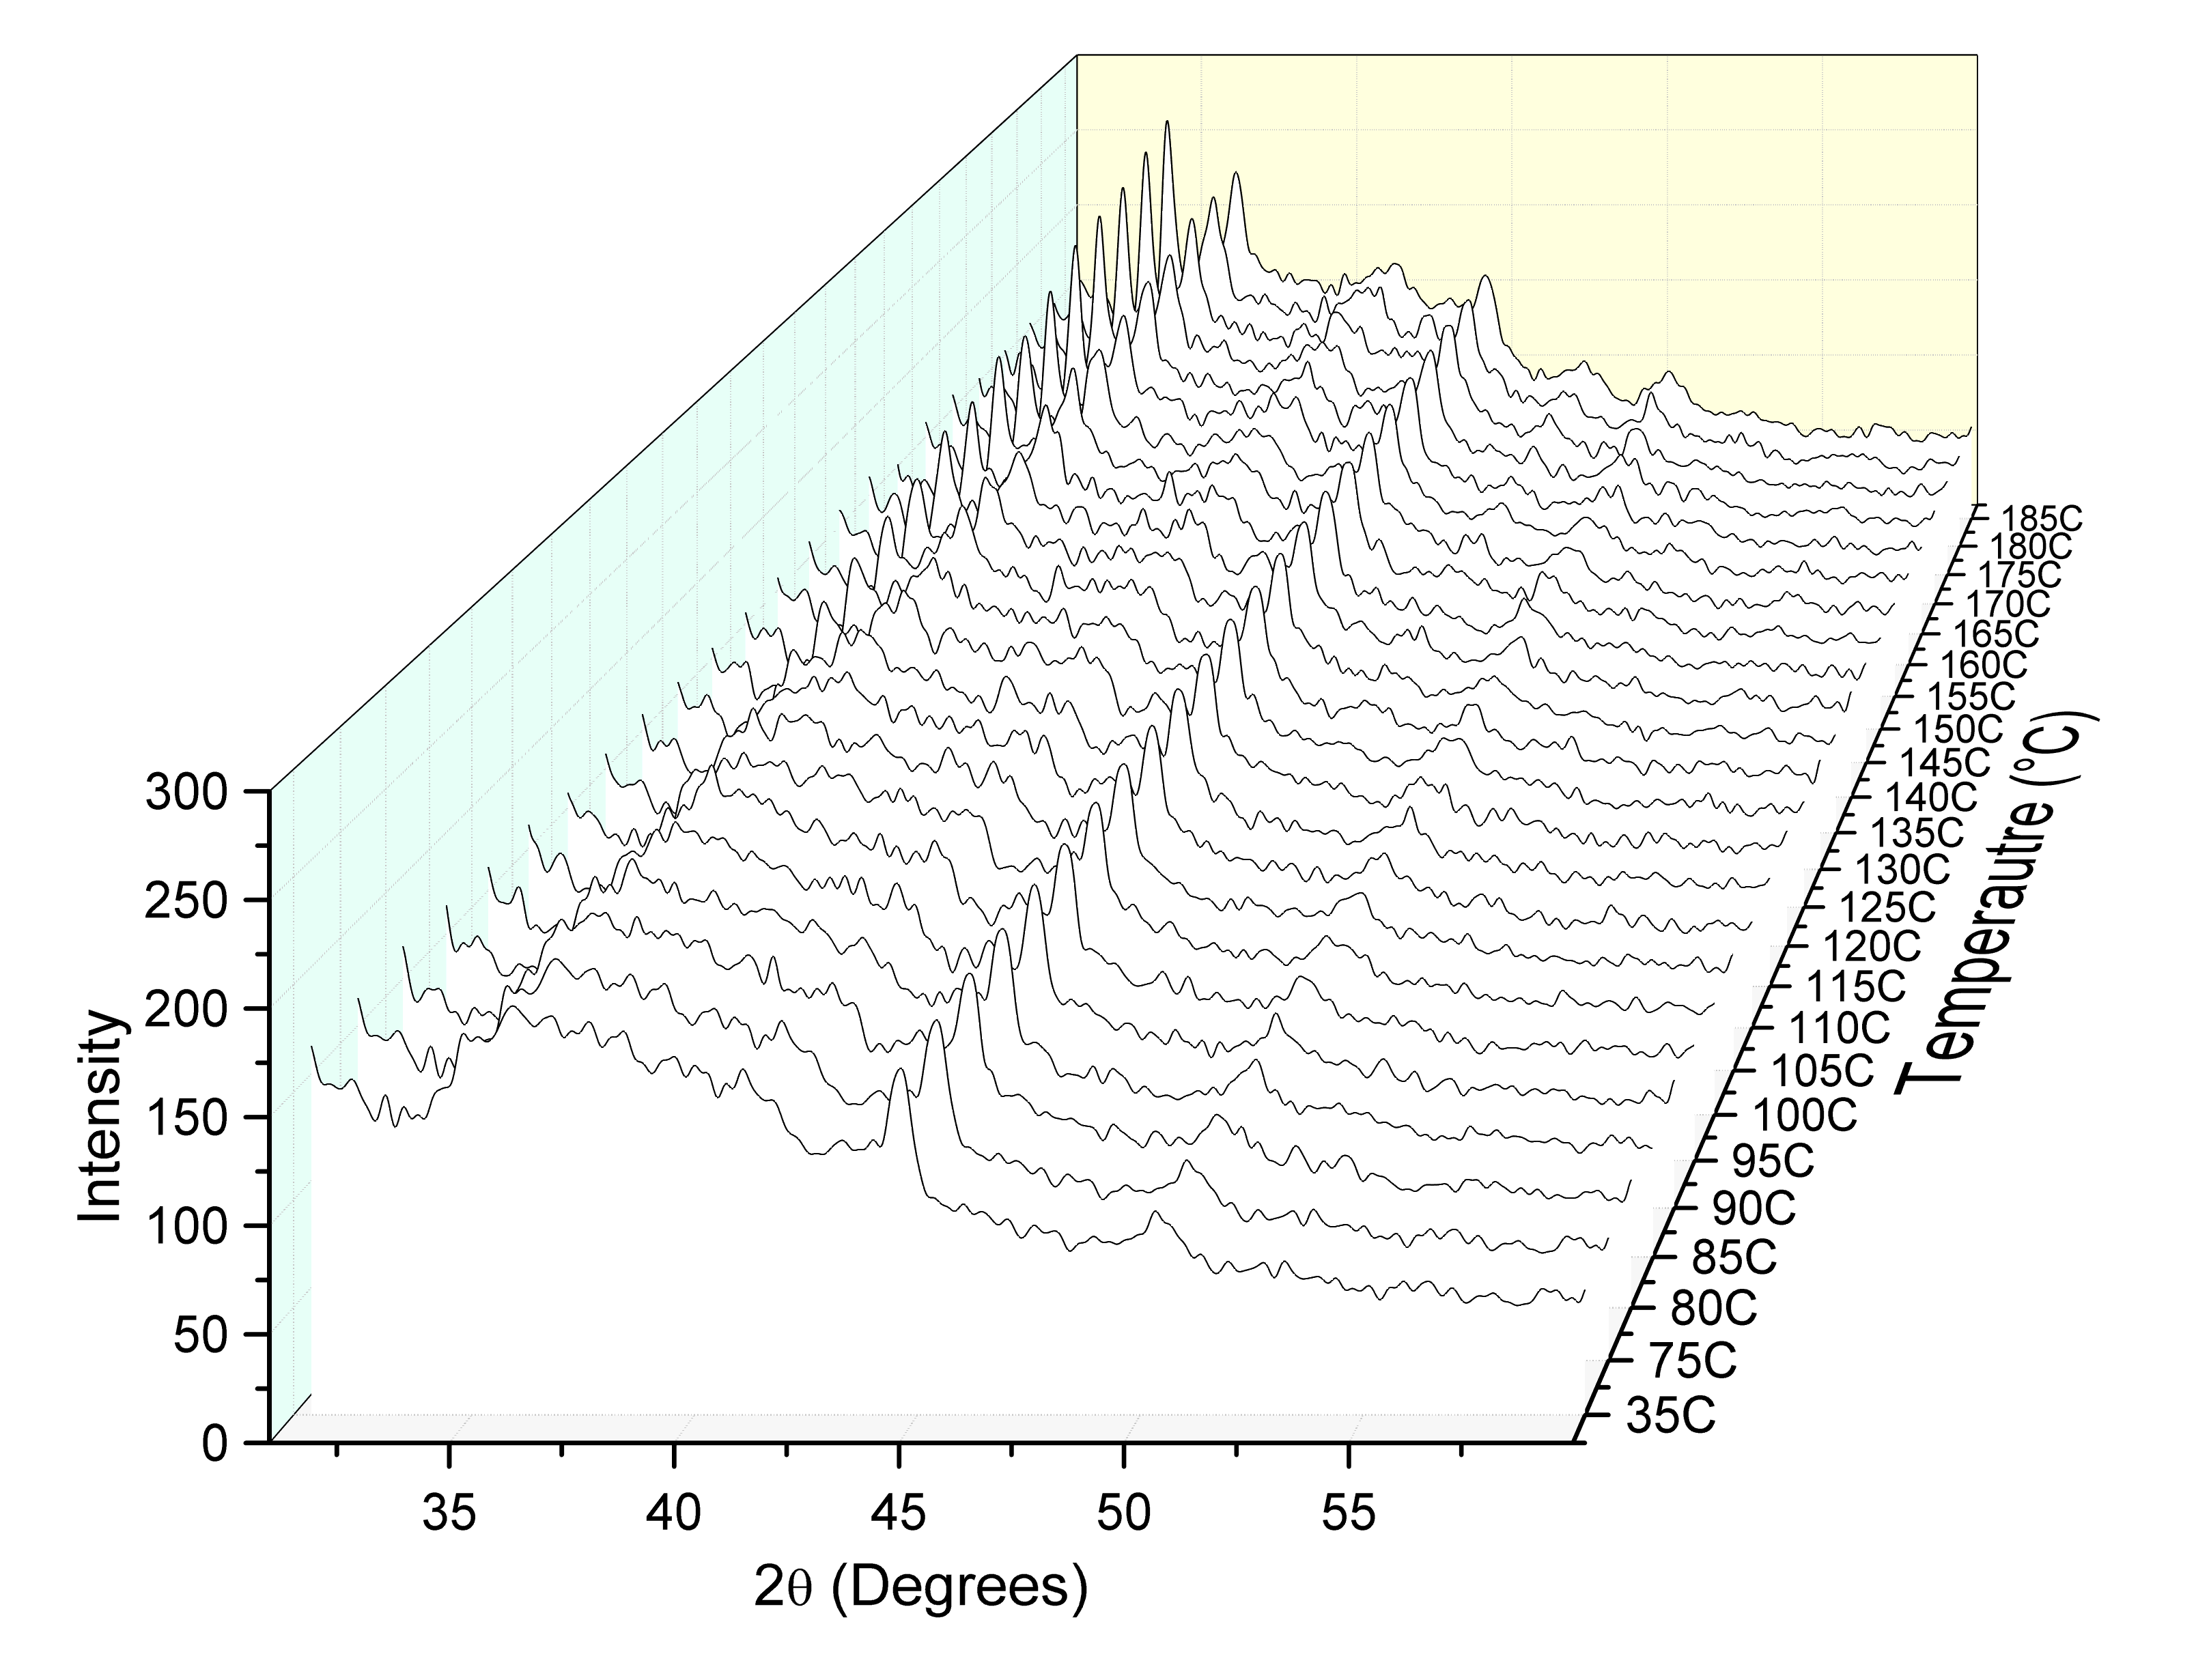
\includegraphics[width=\textwidth]{TF_Facet_HeatXRD_Waterfall3D_Smooth.png}
		\caption{}
		\label{fig:XRD_Dynamic_WaterFall_Film}
	\end{subfigure}
	\caption{(a) Stacked \gls{xrd} patterns from the incremental heating of film \MgZnCa. (b) Cascading \gls{xrd} patterns from the incremental heating of film \MgZnCa. }%global caption
	\label{fig:XRD_Dynamic_Film}
\end{figure}

%%%%%%%%%%%%%%%%%%%%%%%%%%%%%%%%%%%%%%%%%%%%%%%%%%%%%%%%%%%%%%%%%%%%%%%%%%

\section{DISCUSSION}

The use of a 60K \gls{dsc} heating rate compared to the more commonly used 20K rate [sources] shifts peaks for the bulk \MgZnCa~ alloy about 8 - 15 degrees higher. This higher heating rates were used because crystallization events for the films were different to differentiation at the lower heating rate. 
Films show little shift to high temperature peaks with increases heating rates, but large shifts with relaxation. 
Bulk show the opposite behaviour, larger peaks shifts with higher heating rates and little shift with relaxation.

%%%%%%%%%%%%%%%%%%%%%%%%%%%%%%%%%%%%%%%%%%%%%%%%%%%%%%%%%%%%%%%%%%%%%%%%%%

\section{CONCLUSIONS}

%%%%%%%%%%%%%%%%%%%%%%%%%%%%%%%%%%%%%%%%%%%%%%%%%%%%%%%%%%%%%%%%%%%%%%%%%%

\section{ACKNOWLEDGEMENTS}

%People
Yu Wang for his assistance with \acrshort{xrd} experimentation and Rietveld refinement. 

%%%%%%%%%%%%%%%%%%%%%%%%%%%%%%%%%%%%%%%%%%%%%%%%%%%%%%%%%%%%%%%%%%%%%%%%%%

%Bibliography
\bibliography{ThesisBib}
\bibliographystyle{unsrt}

%%%%%%%%%%%%%%%%%%%%%%%%%%%%%%%%%%%%%%%%%%%%%%%%%%%%%%%%%%%%%%%%%%%%%%%%%%


\end{document}